% !TEX program = lualatex
\documentclass[UTF8, a4paper, 12pt]{ctexart}

%% === 导言区：宏包配置 ===
\usepackage{geometry}
\geometry{left=2.5cm,right=2.5cm,top=2.5cm,bottom=2.5cm} % 标准页边距
\usepackage{amsmath, amssymb,amsthm} % 数学公式
\usepackage{graphicx}         % 图片支持
\usepackage{array}
\usepackage{tabularx}
\usepackage{booktabs}         % 顶刊必备：专业三线表
\usepackage{multirow}         % 表格多行合并
\usepackage{makecell}         % 单元格内换行
\usepackage{threeparttable}   % 表格注释环境
\usepackage{subcaption}       % 子图
\usepackage[table]{xcolor}    % 表格颜色高亮 (必须加 table 选项)
\usepackage{hyperref}         % 超链接
\hypersetup{
    colorlinks=true,
    linkcolor=black,
    citecolor=blue,           % 引用显示为蓝色，方便审稿人查看
    urlcolor=blue
}

%% === 正文开始 ===
\begin{document}

%% --- 标题页 ---
% 采用方案一：强调协同与价值，去计算机化，更符合管理/交通顶刊口味
\title{\heiti\zihao{2} 考虑并行作业掩盖效应的港口多模态能源协同调度优化}
\author{}
\date{}
\maketitle

%% --- 第一章：绪论 ---
\section{绪论}
\label{sec:intro}

\subsection{研究背景与动机}
在国际海事组织（International Maritime Organization, IMO）日益严格的环境监管框架下，全球航运业正面临深度脱碳转型的迫切需求。船舶在港期间由辅助柴油发电机产生的污染排放，已成为港口碳减排治理中的重点对象。为此，岸电（Shore Power, SP）与电池换电（Battery Swapping, BS）已逐渐成为绿色港口建设中两类具有代表性的船舶补能技术路径。

岸电技术依托港口固定供电设施，为靠泊船舶直接供电，具有能源成本低、技术成熟度高等优势；但其接入与充电过程通常耗时较长，并受泊位及电力基础设施容量的严格约束。相比之下，电池换电通过快速更换整组电池显著缩短补能时间，为电动和混合动力船舶提供了更高的运营灵活性，但同时伴随着较高的服务费用以及对港口电池库存管理能力的要求。由于两种补能模式在时间效率与成本结构上的互补特性，现实港口运行中逐渐形成了岸电与换电并存的混合服务格局。

在政策和市场的双重驱动下，港口侧电气化需求正快速增长。最新的市场报告显示，全球电动船舶市场预计将在 2025 年至 2030 年间以超过 20\% 的年复合增长率（CAGR）迅速扩张 \cite{Markets2025}。特别是混合动力船舶和纯电动船舶正快速渗透短途海运和内河航运细分市场。这一转型刺激了对港口侧能源基础设施的迫切需求。例如，欧盟的《FuelEU海事法规》明确强制要求集装箱船和客船在 2030 年前使用岸电设施（OPS）\cite{EU2025}。与此同时，新兴的移动换电技术正被部署以克服电动船舶的里程焦虑，这共同创造了一个传统港口难以应对的异质性服务环境。

然而，现有港口运营优化研究在刻画能源补给与装卸作业的协同关系方面仍存在明显不足。多数文献要么聚焦于单一能源资源的配置与调度，要么将能源补给视为独立于核心装卸作业之外的附加环节。这种割裂式建模忽视了能源补给与装卸作业在时间维度上的潜在重叠关系，容易导致对船舶在港停留时间和系统运行成本的系统性高估。此外，在船舶数量增加、运行环境动态化的背景下，相关调度问题呈现出显著的时空耦合特征，传统精确优化方法在计算效率上的局限性日益凸显，难以满足实时决策需求。

\subsection{文献综述}
\label{sec:lit_review}

本节从港口岸电资源调度、电动船舶换电模式以及异质性能源协同调度三个维度，对现有的相关研究进行系统回顾，并指出现有文献的局限性，从而确立本文的研究定位。

\subsubsection{岸电资源配置与泊位联合调度}
岸电（Shore Power, SP）作为降低船舶在港排放的成熟技术，其调度优化一直是绿色港口研究的热点。早期的研究主要聚焦于岸电资源的静态分配问题。随着研究的深入，学者们逐渐认识到岸电资源与泊位资源在时空上的强耦合性。

Dai 等 (2020) \cite{Dai2020} 较早提出了岸电泊位分配问题（BAP-SP），目标是在最小化碳排放的同时最大化岸电桩的利用率。在此基础上，Wang 等 (2024) \cite{Wang2024_SP} 进一步引入了多目标优化框架，利用 NSGA-III 算法协同优化泊位调度与岸电分配，证明了联合调度能显著降低船舶的在港等待时间。然而，上述研究普遍存在一个关键假设：即岸电是唯一的清洁能源来源。这种单一资源的视角忽略了日益增长的移动补能需求，难以应对未来多模态并存的复杂场景。

\subsubsection{电动船舶换电模式与移动补能优化}
与岸电的固定属性不同，电池换电（Battery Swapping, BS）为航运业提供了“以空间换时间”的灵活解决方案。Wu 等 (2020) \cite{Wu2020_Review} 在综述中指出，换电技术特别适用于内河及短途海运的集装箱船与渡轮，能够彻底解决充电时间过长的痛点。

针对换电资源的调度，Zhang 等 (2024) \cite{Zhang2024_Voyage} 针对内河全电动船队提出了基于换电站布局的航次调度模型，验证了换电模式在提升船队周转效率方面的优势。Li 等 (2022) \cite{Li2022_BSS} 则从电网互动的角度，研究了换电站的充放电策略以响应分时电价。尽管这些研究深入探讨了换电技术本身，但大多将视角局限于单纯的换电网络或内河航运，尚未将移动换电资源引入繁忙的深海自动化集装箱码头（ACT）调度体系中。

\subsubsection{异质性能源协同与作业掩盖效应}
在实际港口运营中，岸电（固定、廉价、长时）与换电（移动、昂贵、短时）在技术特征上具有天然的互补性。然而，现有的港口调度文献鲜有将这两种异质性资源纳入统一框架。

Yang 等 (2025) \cite{Yang2025_Hybrid} 最近尝试建立了混合动力拖轮的岸电与燃油联合调度模型，这与本文的思路最为接近，但其研究对象仅限于辅助作业船只（拖轮），且未考虑货物装卸对能源服务的刚性时间窗约束。
更重要的是，现有研究普遍采用串行作业（Sequential Operations）假设 \cite{Agatz2018}，即认为能源补给必须在装卸完成后进行。Fan 等 (2021) \cite{Fan2021} 虽然在 LNG 加注领域验证了并行作业（SIMOPS）的安全性与效率价值，但这一机制尚未被数学化地引入到大规模集装箱码头的能源调度模型中。

综上所述，现有文献在“岸电-换电”异质资源的协同调度以及 SIMOPS 机制的数学建模方面仍存在明显的理论空白。本文的研究正是为了填补这一缺口。

\subsection{并行作业掩盖效应 (SIMOPS)}
现有文献中最显著的缺陷在于对作业流程的串行化假设（Sequential Assumption）。大多数研究 \cite{Agatz2018, Moshref2020} 假设船舶必须先完成货物装卸，随后再进行能源补给。这种串行作业假设在建模上较为简洁，但与实际港口运行情况存在偏离。

在现实操作中，港口往往允许能源补给与货物装卸在时间上部分或完全重叠。在海洋工程和港口安全管理领域，这种作业模式通常被称为并行作业（Simultaneous Operations, SIMOPS）。在允许 SIMOPS 的条件下，只要补能作业在装卸作业窗口内完成，其时间消耗便不会对船舶总体在港停留时间产生额外影响。此时，船舶在港停留时长由装卸作业时间与补能作业时间二者中的较大值决定，而非两者之和。本文将这一由并行作业引发的时间折扣现象称为“作业掩盖效应”（masking effect）。

值得注意的是，SIMOPS 并非本研究的理论假设，而是海事工业界为应对紧张船期而广泛采用的标准操作流程。在 LNG 加注领域，为了最小化船舶周转时间，最新的定量风险评估研究已证实，燃料加注与货物装卸的并行作业是提升港口效率的关键手段 \cite{Fan2021}。在岸电操作领域，根据 IEC/IEEE 80005-1 国际标准 \cite{IEC80005}，岸电连接程序通常在船舶靠泊系缆后立即启动，并贯穿于整个货物作业窗口。SIMOPS 并不意味着无约束的完全并行。其可行性仍然受到设备兼容性、安全规范以及船舶内部作业冲突等因素的制约。本文在建模过程中显式刻画这些操作约束，在保证物理可行性与安全性的前提下，引入并行作业所带来的时间掩盖效应，以更真实地反映港口能源与物流协同运行的本质特征。


基于上述行业规范，本研究构建了表 \ref{tab:lit_review} 所示的对比框架，以直观展示本文与现有研究的区别。

%% --- �� 亮点：顶刊风格的文献对比表 ---
\begin{table}[htbp]
    \centering
    \caption{本文与现有相关研究的特征对比分析}
    \label{tab:lit_review}
    \footnotesize 
    \renewcommand{\arraystretch}{1.4} % 增加行高，更美观
    \begin{threeparttable}
        \resizebox{\textwidth}{!}{%
        \begin{tabular}{l c c c c}
            \toprule
            \textbf{文献来源} & \textbf{能源/物流模式} & \textbf{作业逻辑} & \textbf{求解算法} & \textbf{计算效率 (大规模)} \\
            \midrule
            Agatz et al. (2018) \cite{Agatz2018} & 卡车+无人机 & 串行 (Seq.) & 启发式 & 中等 \\
            Moshref-Javadi (2020) \cite{Moshref2020} & 多回路协同 & 串行 (Seq.) & 精确算法 (B\&C) & 低 (N=20) \\
            Roberti \& Ruthmair (2021) & 混合配送 & 串行 (Seq.) & 精确算法 (B\&P) & 低 \\
            \textbf{Hong et al. (2025)} \cite{Hong2025} & \textbf{混合自提网络} & \textbf{串行 (Seq.)} & \textbf{ALNS / Gurobi} & \textbf{低 (N=50, >2600s)} \\
            \midrule
            \rowcolor{gray!15} \textbf{本文 (Ours)} & \textbf{岸电+换电} & \textbf{并行 (SIMOPS)} & \textbf{列生成（CG）} & \textbf{高 (N=100, $\approx$41s)} \\
            \bottomrule
        \end{tabular}%
        }
        \begin{tablenotes}
            \item[注] 粗体部分表示本文的核心改进点；SIMOPS: Simultaneous Operations；Seq.: Sequential。
        \end{tablenotes}
    \end{threeparttable}
\end{table}

如表 \ref{tab:lit_review} 所示，尽管 \cite{Hong2025} 等学者在混合物流调度方面做出了卓越贡献，但其模型仍未考虑作业间的掩盖效应，且其采用的传统求解器或元启发式算法在大规模算例下表现出明显的计算瓶颈。

\subsection{算法挑战：打破计算瓶颈}
在大规模动态港口环境中对 SIMOPS 进行建模引入了复杂的时空耦合约束。虽然精确算法（如分支定价算法 B\&P）理论上能找到最优解，但其搜索空间随船舶数量呈指数级爆炸，在大规模实例中往往面临严重的计算瓶颈。

已有研究指出\textbf{Hong et al. (2025)} \cite{Hong2025} 即便借助商业求解器（如 Gurobi），在包含数十个服务对象的混合调度问题中，求解时间也可能达到数千秒量级。这种计算延迟使得精确算法难以直接应用于具有随机到达、滚动决策特征的实际港口运行环境。为缓解计算压力，部分文献转而采用启发式或元启发式方法以获取可行解，但此类方法通常无法提供最优性保证，且对参数调节和问题规模较为敏感。

上述困境反映了港口与运输调度领域中一个更为普遍的方法论挑战：在满足实时响应需求的前提下，如何在计算可行性与解的最优性之间取得平衡。针对这一问题，本文在保持精确优化框架的基础上，采用列生成（Column Generation, CG）等分解思想缓解计算瓶颈，以提升大规模实例下的求解效率。

\subsection{本文贡献}
针对上述挑战，本文构建了一个考虑 SIMOPS 效应的混合整数规划模型，并提出了一种基于列生成（Column Generation, CG）的精确求解框架。本文的主要贡献总结如下：
\begin{enumerate}
    \item \textbf{模型创新：} 首次将 SIMOPS 机制引入港口能源调度，建立了显式包含 $T_{stay} = \max(T_{cargo}, T_{energy})$ 约束的数学模型，量化了并行作业带来的成本节约与效率提升。
    \item \textbf{算法创新：}提出一种列生成求解框架，通过主问题与定价子问题的分解，在保证精确优化求解结构的前提下缓解大规模实例下的计算复杂度。
    \item \textbf{实证突破：}基于大规模异质性算例的数值实验结果表明，所提出的列生成框架在解质量与计算效率之间实现了良好平衡，验证了其在实际港口调度场景中的应用潜力。
\end{enumerate}
%% ==============================================================
%% SECTION 2: PROBLEM DESCRIPTION AND MODEL
%% ==============================================================

%% ==============================================================
%% SECTION 2: PROBLEM DESCRIPTION AND MODEL (FINAL ACADEMIC VERSION)
%% ==============================================================

%% ==============================================================
%% SECTION 2: PROBLEM DESCRIPTION AND MODEL (NARRATIVE FLOW VERSION)
%% ==============================================================

\section{问题描述与数学建模}
\label{sec:model}

\subsection{问题定义与决策结构}
\label{sec:problem_definition_cn}

本文研究的是自动化集装箱码头环境下的港口能源—作业协同调度问题。在船舶靠泊期间，港口运营方需要在满足装卸作业需求的同时，为船舶提供能源服务，并合理协调能源服务选择、资源占用以及船舶离港时序，其目标是最小化包含能源成本、碳排放外部性以及时间机会成本在内的广义运营成本。

从运筹优化的角度来看，该问题可被抽象为一类具有\emph{异质性服务选项}和\emph{异质性延误惩罚}的港口调度问题。在该问题中，能源补给不再被视为独立于装卸作业之外的附属环节，而是与船舶在港停留时间直接耦合的关键决策变量。这一建模视角与近年来将港口视为综合物流—能源系统的研究趋势一致 \cite{andersson2017shipping,bergqvist2019ports}。

在所考虑的系统中，港口运营中心（Terminal Operating Center, TOC）在船舶到达港口后，需要在多个可行的能源服务选项之间为其做出选择，并同时确定能源服务的开始时刻。该决策过程受到港口能源基础设施容量约束、船舶作业时间窗以及船舶对离港延误的异质性敏感程度等多重因素的共同影响。

与大量现有港口与运输调度文献不同，本文允许能源服务与货物装卸作业在时间维度上发生重叠。现有研究普遍采用串行作业假设，即认为船舶必须在完成装卸作业后才能开始能源补给。尽管该假设在建模上较为简洁，但已有研究指出，其可能系统性高估船舶在港停留时间，从而影响资源配置与调度决策的合理性 \cite{agatz2018tsp,moshref2020multi}。

从问题结构上看，本文研究的是一个\emph{服务选择—排队—离港时序联合优化问题}，其主要特征体现在以下几个方面。

首先，能源服务选项在资源占用方式、服务持续时间以及成本结构方面具有显著的结构异质性。这使得港口能源调度问题不同于传统的单资源或单机器调度问题，而更接近于具有多种服务类型和容量约束的调度问题 \cite{brucker2007scheduling}。如图\ref{fig:scenario} 所示，在港口能源系统中，岸电服务依赖固定泊位和电力基础设施，换电服务依赖移动设备，而传统燃油模式则不消耗任何港口外部资源。

\begin{figure}[htbp]
    \centering
    \includegraphics[width=1.0\textwidth]{Fig1_Port_Scenario.png}
    \caption{\textbf{港口多模态能源调度场景示意图。} 图中直观展示了三种异质性服务模式：(Left) 岸电模式受限于固定桩位；(Middle) 换电模式受限于移动车辆数；(Right) 燃油辅机模式作为无资源约束的保底选项。所有模式均与装卸作业并行 (SIMOPS)。}
    \label{fig:scenario}
\end{figure}


其次，船舶在时间价值上的异质性被显式纳入决策结构。本文通过为不同船舶设置差异化的延误惩罚系数，刻画其对离港延误的敏感程度。这种建模方式与调度理论中关于异质性迟到惩罚（heterogeneous tardiness penalties）的研究方向保持一致，其优势在于能够通过成本权衡内生决定服务优先级，而无需人为设定固定优先规则 \cite{pinedo2016scheduling,vidal2013heuristics}。

再次，该问题具有明显的动态调度与资源竞争特征。在船舶随机到达且能源服务容量有限的条件下，排队等待将直接影响船舶的离港时刻，进而影响系统总体运营成本。因此，该问题在结构上更接近于带时间维度和资源竞争约束的动态调度问题，而非静态分配模型 \cite{brucker2006complexity,cordeau2015transportation}。

综合上述分析，本文所研究的问题可概括为：在允许能源服务与装卸作业并行的条件下，对具有异质性延误惩罚的船舶进行能源服务选择与时序调度，以最小化系统整体运营成本。尽管已有研究分别探讨了港口能源管理、混合服务调度以及并行作业在特定工程场景下的可行性，但将上述要素统一纳入一个精确优化框架加以系统刻画的研究仍然较为有限。本文正是从这一结构性空白出发，对港口能源—作业协同调度问题进行建模与分析。


\subsection{能源服务类型与资源特征}
\label{sec:energy_service_types}

在港口能源—作业协同调度问题中，能源服务并非同质资源，而是由多种在资源占用方式、服务时长和成本结构上均存在显著差异的服务类型构成。本文将港口可提供的能源补给方式统一建模为一组\emph{具有不同资源特征的服务选项}，从而在统一优化框架下刻画其对调度决策的影响。

具体而言，本文考虑以下三类能源服务类型。

\paragraph{岸电服务（Shore Power, SP）}
岸电服务通过固定岸电桩将港口电网直接连接至船舶，为其在港期间提供持续电力支持。该服务模式在单位能源成本和碳排放水平方面具有显著优势，因此被视为绿色港口建设中的核心技术之一。相关研究表明，岸电在降低港口区域空气污染和温室气体排放方面具有明确成效 \cite{andersson2017shipping,bergqvist2019ports}。

从调度角度看，岸电服务具有以下关键特征：  
(1) 其服务过程依赖于稀缺的固定基础设施资源（岸电桩及对应泊位）；  
(2) 服务持续时间通常较长，且与船舶能源需求和供电功率直接相关；  
(3) 当岸电资源被占用时，新到船舶需产生排队等待时间。

因此，在优化模型中，岸电服务被刻画为一种\emph{具有时间跨度和容量约束的资源消耗型服务}，其使用将直接影响其他船舶的可行服务时序。

\paragraph{换电服务（Battery Swapping, BS）}
换电服务通过移动换电设备为船舶快速更换整组电池，从而在极短时间内完成能源补给。与岸电相比，换电服务在时间维度上具有显著优势，能够有效降低船舶在港停留时间，尤其适用于对时间敏感度较高的船舶类型。近年来，换电被视为解决电动船舶“里程焦虑”和提升港口运行灵活性的重要手段 \cite{wu2020battery,zhang2022maritime}。

在资源特征上，换电服务与岸电存在本质差异：  
(1) 其服务依赖于有限数量的移动换电设备，而非固定泊位；  
(2) 服务时长较短，通常可近似视为瞬时或准瞬时操作；  
(3) 单位服务成本相对较高，反映了设备投入和电池管理成本。

在模型中，换电服务被视为一种\emph{占用时间短但容量受限的高成本服务选项}，其存在为调度问题引入了“以成本换时间”的权衡路径。

\paragraph{褐色服务（燃油辅机，Brown-AE）}
褐色服务指船舶在港期间完全依赖自身燃油辅机完成能源供给。该服务模式不消耗任何港口侧能源基础设施资源，因此在调度上不受容量约束，也不会引发排队等待。然而，其能源成本和碳排放成本显著高于绿色能源选项，与当前港口低碳发展目标存在冲突。

从运筹建模角度来看，褐色服务在本文中扮演着\emph{保底服务选项（fallback option）}的角色。类似的建模思想在运输与生产调度文献中常被用于刻画外包服务、应急资源或惩罚性松弛机制 \cite{cordeau2015transportation,pinedo2016scheduling}。通过引入褐色服务，模型在任何负载水平下均可保持可行性，同时通过高昂的成本惩罚，引导系统在条件允许时优先选择绿色能源方案。

\paragraph{服务类型的结构性差异}
综上所述，三类能源服务在资源占用方式、服务持续时间以及成本结构方面具有显著差异。岸电服务体现为\emph{长时、低成本、强容量约束}的服务类型；换电服务体现为\emph{短时、高成本、弱容量约束}的服务类型；褐色服务则体现为\emph{零等待、高成本、无容量约束}的服务类型。

这种服务异质性是本文调度问题复杂性的核心来源之一，也使得该问题区别于传统单资源调度或单服务排队模型。通过将上述能源补给方式统一建模为具有不同资源轮廓的服务选项，本文为后续刻画并行作业（SIMOPS）机制以及构建精确优化模型奠定了基础。


\subsection{并行作业与完工时间耦合结构（SIMOPS）}
\label{sec:simops_structure}

本文的核心建模特征在于显式引入能源服务与货物装卸作业的并行作业机制（Simultaneous Operations, SIMOPS），并据此刻画船舶在港停留时间的结构性变化。在传统港口调度模型中，装卸作业与能源补给通常被假设为严格串行过程，即船舶需在完成装卸作业后方可进行能源服务。在该假设下，船舶在港停留时间可表示为装卸时间与能源服务时间的加性函数。

然而，实际港口运行中，上述串行假设往往过于保守。在满足安全规范和设备兼容性要求的前提下，港口通常允许船舶在装卸作业进行的同时完成能源补给。这种并行作业模式在海洋工程和港口安全管理领域被称为并行作业（SIMOPS），并已在液化天然气（LNG）加注、岸电连接等场景中得到广泛应用和验证 \cite{fan2021simops,IEC80005}。

\begin{figure}[htbp]
    \centering
    % 请确保文件名一致，宽度设置为页面的 90%
    \includegraphics[width=0.95\textwidth]{Fig_Gantt_Enhanced.png}
    \caption{\textbf{SIMOPS 掩盖效应机制可视化甘特图。} 灰色区域代表刚性的货物装卸窗口，绿色条代表岸电补能时间。对于 Ship 0, 1, 2, 4，补能时间完全被装卸窗口“掩盖”，未产生额外延误；对于 Ship 3，由于装卸窗口过短，系统智能切换为换电模式（红色）以减少滞港时间。}
    \label{fig:masking_mechanism}
\end{figure}
掩盖效应（Masking Effect）的经济学解释：
结合图 \ref{fig:masking_mechanism} 可以直观地看出：
 \textbf{完全掩盖 (Fully Masked)}：如 Ship 0 所示，当 $T_{service} \le T_{cargo}$ 时，能源服务的边际时间成本为零。
 \textbf{模式切换 (Mode Switching)}：如 Ship 3 所示，当装卸时间不足以覆盖岸电充电时，为了避免延误，模型会自动选择换电模式。

\paragraph{完工时间结构的变化}
引入 SIMOPS 后，船舶在港停留时间不再由各作业时间的简单累加决定，而是由装卸作业与能源服务中较长者主导。设船舶 $i$ 的装卸作业时长为 $T^{(i)}_{\text{cargo}}$，能源服务所需时长为 $T^{(i)}_{\text{service}}$，排队等待时间为 $W_i$，则其实际在港停留时间可表示为：
\begin{equation}
T^{(i)}_{\text{stay}} = \max \left\{ T^{(i)}_{\text{cargo}},\; T^{(i)}_{\text{service}} \right\} + W_i .
\label{eq:simops_max}
\end{equation}

式 \eqref{eq:simops_max} 表明，并行作业机制将船舶完工时间的结构从\emph{加性形式}转变为\emph{瓶颈主导（bottleneck-driven）的最大值形式}。当能源服务能够在装卸作业窗口内完成时，其时间消耗将被装卸作业“掩盖”，不会对船舶离港时刻产生额外影响。本文将这一现象称为\emph{作业掩盖效应（masking effect）}。

从调度理论角度来看，该结构性变化具有重要意义。大量经典调度模型基于作业时间可加的假设，而最大值形式的完工时间函数会显著改变问题的可行域和目标函数形态，从而影响问题的计算复杂性和求解策略 \cite{brucker2007scheduling,pinedo2016scheduling}。

\paragraph{并行作业的可行性与约束}
需要强调的是，SIMOPS 并不意味着无约束的完全并行。在实际港口环境中，并行作业的可行性受到多种因素制约，包括但不限于设备兼容性、作业安全规范以及船舶内部作业冲突。相关研究表明，在合理的风险评估和操作规程约束下，并行作业不仅是可行的，而且是提升港口效率的重要手段 \cite{fan2021simops}。

在岸电操作领域，IEC/IEEE~80005-1 国际标准明确规定，岸电连接流程可在船舶靠泊并完成系缆后启动，并贯穿于货物装卸全过程 \cite{IEC80005}。因此，在本文模型中，SIMOPS 被视为一种符合现实操作规范的作业机制，而非理想化假设。

\paragraph{SIMOPS 对调度决策的影响}
SIMOPS 机制的引入不仅改变了船舶完工时间的计算方式，也深刻影响了调度决策的权衡逻辑。具体而言，在并行作业条件下，延长能源服务时间并不一定导致船舶离港延误，这使得低成本但服务时间较长的能源选项在某些情况下具有更高的吸引力。相反，当装卸作业窗口较短或能源资源拥挤导致排队等待时，高效率但成本较高的服务选项可能成为更优选择。

这种由 SIMOPS 引发的非线性权衡关系，使得能源服务选择、排队行为和离港时序高度耦合，也构成了本文调度问题区别于传统串行调度模型的核心特征。后续的数学模型将围绕式 \eqref{eq:simops_max} 所刻画的完工时间结构展开，并在此基础上构建精确的优化框架。


\subsection{数学模型与线性化}
\label{sec:model_formulation}

本节在第~\ref{sec:problem_definition_cn}--\ref{sec:simops_structure} 节问题定义与并行作业（SIMOPS）机制的基础上，
构建港口能源--作业协同调度问题的混合整数线性规划（MILP）模型。
为避免使用大 $M$ 线性化并增强模型松弛强度，
本文采用基于\emph{服务开始时刻指示变量}的时间展开（time-indexed）建模方式。
\subsubsection{时空网络结构建模}

港口能源--作业协同调度问题本质上涉及多艘船舶在时间与空间维度上
对有限能源资源的动态竞争关系。
不同船舶的服务开始时刻、资源占用行为以及离港时间
通过容量约束与并行作业机制发生耦合，
从而构成一个具有显著时空关联特征的调度系统。
上述特征决定了有必要在形式化建模之前，
对问题的内在结构进行结构化刻画。

为刻画上述结构性关联，
本文将问题表示为一张有向时空网络
$G=(\mathcal{V},\mathcal{A})$，
其中节点集合 $\mathcal{V}$ 对应于待调度船舶集合 $\mathcal{N}$，
用于刻画船舶层面的决策单元；
弧集合 $\mathcal{A}$ 则用于表示船舶之间
因资源竞争与时间可行性约束所产生的潜在相互影响关系。

\paragraph{节点与特征表示}
对于任意节点 $i\in\mathcal{V}$，
定义其特征向量 $h_i$ 用以描述船舶的关键属性与调度状态：
\begin{equation}
h_i =
\big[
A_i,\,
D_i,\,
E_i,\,
T^{(i)}_{\text{cargo}},\,
Loc_i,\,
Type_i,\,
C^{(i)}_{\text{delay}}
\big]^{\top}.
\end{equation}
其中，
$Loc_i$ 表示船舶的泊位或空间位置特征，
$Type_i$ 为能源兼容性的类别编码（如是否支持岸电）。
该特征向量刻画了船舶在调度决策中的局部环境与约束条件，
其各组成元素均直接来源于后续数学模型中的参数或变量设定，
从而保证表示层与优化模型之间的一致性。

\paragraph{弧的定义与可行性约束}
图中的有向弧 $(i,j)\in\mathcal{A}$ 用于表示
在时间与资源约束条件下，
船舶 $j$ 的能源服务或装卸作业
可能受到船舶 $i$ 决策的影响。
对于可移动能源资源（如换电设备），
若其可在完成对船舶 $i$ 的服务后转移至船舶 $j$，
则需满足如下时间可行性约束：
\begin{equation}
S_i + T^{(i)}_{\text{serv}} + T^{(i,j)}_{\text{travel}} \le S_j ,
\end{equation}
其中 $T^{(i,j)}_{\text{travel}}$ 表示资源在两艘船舶之间的转移时间。
该连续时间关系用于描述问题的结构特征，
其在后续数学模型中将通过离散时间展开变量进行刻画，
并对应于离散服务时长 $d_i^{SP}$ 或 $d_i^{BS}$。
对于固定能源资源（如岸电桩），
弧的构造则反映了基于空间位置与容量限制的冲突关系。

\paragraph{结构化表示的意义}
通过上述时空网络建模，
原问题中的资源容量约束与时间耦合关系
被显式嵌入于图结构之中。
需要强调的是，
该网络表示并不意味着问题被严格等价地转化为
标准的网络流模型，
而是一种用于刻画资源与时间耦合关系的结构化抽象。
该表示方式为后续采用列生成方法刻画资源竞争提供了结构基础，
同时也为在结构化表示之上引入学习方法以加速求解过程奠定了表示层基础。



% ------------------------------------------------
% 2.4.1 集合、参数与变量
% ------------------------------------------------
\subsubsection{集合、参数与变量}

\begin{table}[htbp]
\centering
\caption{集合与索引定义}
\begin{tabular}{ll}
\toprule
符号 & 含义 \\
\midrule
$\mathcal{N}$ & 规划期内待服务船舶集合，索引 $i \in \mathcal{N}$ \\
$\mathcal{K}^{SP}$ & 岸电桩集合，索引 $k \in \mathcal{K}^{SP}$ \\
$\mathcal{K}^{BS}$ & 换电设备集合（同质资源），$|\mathcal{K}^{BS}| = K^{BS}$ \\
$\mathcal{T}$ & 离散时间段集合，索引 $t \in \mathcal{T}$ \\
\bottomrule
\end{tabular}
\end{table}


\begin{table}[htbp]
\centering
\caption{模型参数定义}
\begin{tabular}{ll}
\toprule
参数 & 含义 \\
\midrule
$A_i$ & 船舶 $i$ 的到达时间（时间段索引） \\
$D_i$ & 船舶 $i$ 的期望离港截止时间（时间段索引） \\
$T^{(i)}_{\text{cargo}}$ & 船舶 $i$ 的装卸作业时长（时间段数） \\
$E_i$ & 船舶 $i$ 的能源需求量 \\
$P^{SP}$ & 岸电供电功率 \\
$T^{BS}$ & 换电服务持续时间（时间段数） \\
$C^{SP}$ & 单位岸电能源成本 \\
$C^{BS}$ & 换电服务固定成本 \\
$C^{AE}$ & 褐色模式单位能源与排放综合成本 \\
$C^{(i)}_{\text{delay}}$ & 船舶 $i$ 的单位延误惩罚系数 \\
$Q_{ik}$ & 船舶 $i$ 与岸电桩 $k$ 的兼容性参数（0/1） \\
$K^{BS}$ & 换电设备数量（$K^{BS}=|\mathcal{K}^{BS}|$） \\
\bottomrule
\end{tabular}
\end{table}


\begin{table}[htbp]
\centering
\caption{决策变量定义}
\begin{tabular}{ll}
\toprule
变量 & 含义 \\
\midrule
$x_{ik} \in \{0,1\}$ & 若船舶 $i$ 选择岸电桩 $k$，则取 1 \\
$y_i \in \{0,1\}$ & 若船舶 $i$ 选择换电服务，则取 1 \\
$z_i \in \{0,1\}$ & 若船舶 $i$ 选择褐色服务，则取 1 \\
$w_{it} \in \{0,1\}$ & 若船舶 $i$ 在时间段 $t$ 开始能源服务，则取 1 \\
$u_{ikt} \in \{0,1\}$ & 若船舶 $i$ 在时间段 $t$ 占用岸电桩 $k$，则取 1 \\
$v_{it} \in \{0,1\}$ & 若船舶 $i$ 在时间段 $t$ 正在进行换电服务，则取 1 \\
$L_i \ge 0$ & 船舶 $i$ 的实际离港时间（时间段索引） \\
$\delta_i \ge 0$ & 船舶 $i$ 的延误量 \\
\bottomrule
\end{tabular}
\end{table}


% ------------------------------------------------
% 2.4.2 目标函数
% ------------------------------------------------
\subsubsection{目标函数}

模型目标是在满足资源容量与作业约束的前提下，
最小化系统广义运营总成本：
\begin{equation}
\min Z =
\sum_{i \in \mathcal{N}}
\Big(
C^{SP} E_i \sum_{k \in \mathcal{K}^{SP}} x_{ik}
+ C^{BS} y_i
+ C^{AE} E_i z_i
\Big)
+ \sum_{i \in \mathcal{N}} C^{(i)}_{\text{delay}} \delta_i .
\label{eq:obj_24_final}
\end{equation}

% ------------------------------------------------
% 2.4.3 约束条件
% ------------------------------------------------
\subsubsection{约束条件}

\paragraph{(1) 服务模式选择约束}
\begin{equation}
\sum_{k \in \mathcal{K}^{SP}} Q_{ik} x_{ik} + y_i + z_i = 1,
\quad \forall i \in \mathcal{N}.
\label{eq:mode_24_final}
\end{equation}

\paragraph{(2) 能源服务开始时刻约束}
若船舶 $i$ 选择岸电或换电服务，则必须且只能在某一时间段开始能源服务：
\begin{equation}
\sum_{t \in \mathcal{T}} w_{it}
=
\sum_{k \in \mathcal{K}^{SP}} x_{ik} + y_i,
\quad \forall i \in \mathcal{N}.
\label{eq:w_unique_24}
\end{equation}

\paragraph{(3) 服务持续时间定义}
\begin{equation}
d_i^{SP} = \left\lceil \frac{E_i}{P^{SP}} \right\rceil, 
\qquad
d_i^{BS} = T^{BS}.
\label{eq:duration_24}
\end{equation}

\paragraph{(4) 岸电占用链接约束}
\begin{equation}
u_{ikt}
=
\sum_{\tau = \max\{0,\, t-d_i^{SP}+1\}}^{t}
w_{i\tau} \cdot x_{ik},
\quad \forall i,k,t.
\label{eq:link_sp_24_final}
\end{equation}

\paragraph{(5) 换电占用链接约束}
\begin{equation}
v_{it}
=
\sum_{\tau = \max\{0,\, t-d_i^{BS}+1\}}^{t}
w_{i\tau} \cdot y_i,
\quad \forall i,t.
\label{eq:link_bs_24_final}
\end{equation}

\paragraph{(6) 资源容量约束}
\begin{align}
\sum_{i \in \mathcal{N}} \sum_{k \in \mathcal{K}^{SP}} u_{ikt}
&\le |\mathcal{K}^{SP}|,
&& \forall t \in \mathcal{T},
\label{eq:cap_sp_24_final} \\
\sum_{i \in \mathcal{N}} v_{it}
&\le K^{BS},
&& \forall t \in \mathcal{T}.
\label{eq:cap_bs_24_final}
\end{align}

\paragraph{(7) SIMOPS 完工时间约束}
\begin{align}
L_i &\ge A_i + T^{(i)}_{\text{cargo}},
&& \forall i \in \mathcal{N},
\label{eq:cargo_finish_24_final} \\
L_i &\ge 
\sum_{t \in \mathcal{T}} t \cdot w_{it}
+ d_i^{SP}\sum_{k \in \mathcal{K}^{SP}} x_{ik}
+ d_i^{BS} y_i,
&& \forall i \in \mathcal{N}.
\label{eq:service_finish_24_final}
\end{align}

\paragraph{(8) 延误量线性化}
\begin{align}
\delta_i &\ge L_i - D_i,
&& \forall i \in \mathcal{N}, \\
\delta_i &\ge 0,
&& \forall i \in \mathcal{N}.
\end{align}

\paragraph{(9) 变量域约束}
\begin{equation}
x_{ik},y_i,z_i,w_{it},u_{ikt},v_{it} \in \{0,1\},
\quad
L_i,\delta_i \ge 0.
\end{equation}

\subsection{模型性质与特例分析}
\label{sec:properties}

本节从运筹优化角度对前述模型的若干关键性质进行讨论，并分析其在特定参数设定下与已有经典调度问题之间的关系。相关分析有助于理解问题的结构复杂性，并为后续求解方法的设计提供理论依据。

\subsubsection{SIMOPS 机制下的完工时间结构性质}

引入并行作业（SIMOPS）机制后，船舶在港停留时间由装卸作业与能源服务中较长者主导，其完工时间由加性结构转变为最大值结构。该性质在模型中通过约束
\eqref{eq:cargo_finish_24_final}--\eqref{eq:service_finish_24_final} 实现。

这一结构变化带来两个重要影响。首先，能源服务时长并非总是直接影响船舶离港时间。当能源服务能够在装卸作业窗口内完成时，其时间消耗将被装卸作业完全掩盖，从而不会引发额外延误。其次，服务时长与离港时间之间的非线性关系使得调度决策不再遵循“服务越快越优”的单调逻辑，而是取决于装卸窗口、资源竞争以及延误惩罚之间的综合权衡。

从调度理论视角来看，该最大值完工时间结构显著区别于传统可加调度模型，并会改变问题的可行域形态和对偶价格结构，这也是后续采用列生成与路径定价思想的重要动因。

\subsubsection{保底服务选项与模型可行性}

模型中引入的褐色服务模式不依赖港口侧能源资源，因此不受容量约束限制。在优化结构上，该服务模式可被视为一种\emph{保底服务选项（fallback option）}，其主要作用体现在两个方面。

一方面，褐色服务保证了模型在任意船舶到达负载和资源容量配置下的可行性，避免了因能源资源不足导致的不可行解。另一方面，通过在目标函数中施加较高的单位成本，模型能够在保证可行性的同时，引导系统在资源允许的条件下优先选择绿色能源服务。

类似的建模思想在运输与生产调度文献中常被用于刻画外包服务、应急资源或罚函数松弛机制，其引入往往有助于平衡模型的可行性与经济合理性。

\subsubsection{异质性延误惩罚的结构影响}

模型通过船舶特定的延误惩罚系数刻画其对离港延误的异质性敏感程度。在该框架下，船舶并未被赋予外生的优先级规则，而是通过目标函数中的成本权衡内生决定其服务选择和等待行为。

当延误惩罚系数较大时，模型倾向于为船舶分配效率更高的能源服务选项或减少其排队等待时间；反之，当延误惩罚较小时，船舶更可能选择低成本但服务时长较长的能源服务模式。该结构使得不同船舶在相同资源环境下表现出差异化的调度结果，从而增强了模型对现实运营行为的刻画能力。

\subsubsection{问题复杂性与规模增长特性}

尽管本文模型在形式上属于混合整数线性规划，其组合复杂性仍随船舶数量和时间离散粒度的增加迅速增长。特别地，时间展开变量 $w_{it}$、$u_{ikt}$ 和 $v_{it}$ 的引入，使得变量数量与时间段数呈线性关系，从而在大规模实例下导致模型规模显著膨胀。

此外，SIMOPS 机制引入的完工时间最大值结构以及多类服务选项的并存，使得问题同时具备服务选择、排队竞争和时序优化等多重组合特征。上述因素共同表明，该问题在计算上具有较高复杂性，难以通过直接求解大规模 MILP 获得高质量解，这为后续采用分解算法和近似加速策略提供了现实动机。

\subsubsection{特例分析}

在特定参数或约束设定下，本文模型可退化为若干已有的经典调度问题。

\paragraph{(1) 串行作业特例}
当不允许能源服务与装卸作业并行时，完工时间结构退化为装卸时间与能源服务时间的加性形式。此时，模型可视为一类带异质性延误惩罚的服务选择与排队调度问题，其结构与传统串行港口调度模型一致。

\paragraph{(2) 纯绿色能源特例}
当禁止褐色服务模式（即 $z_i=0,\ \forall i$）时，模型退化为一个纯绿色能源调度问题。在该情形下，所有船舶必须在有限岸电和换电资源之间竞争，从而凸显能源基础设施容量配置对系统性能的影响。

\paragraph{(3) 同质船舶特例}
当所有船舶的延误惩罚系数相同，且能源需求与装卸时长一致时，模型退化为同质船舶调度问题。此时，异质性因素消失，调度结果主要由资源容量和服务效率决定。

\paragraph{(4) 单一能源服务特例}
当仅允许一种能源服务类型（例如仅岸电）时，模型进一步退化为具有并行作业特征的单资源调度问题。

上述特例分析表明，本文提出的模型可被视为一个统一的调度框架，能够在不同参数设定下涵盖多类已有问题，并通过引入 SIMOPS 机制与多服务选项扩展了传统港口调度模型的适用范围。


\section{数值实验}
\label{sec:computational}

本章通过数值实验系统评估所提出的“考虑 SIMOPS 掩盖效应的港口多模态能源协同调度模型”及其列生成（CG）求解框架的有效性与可扩展性，重点回答以下问题：
(1) SIMOPS 掩盖效应在成本与效率层面的量化收益有多大？
(2) 与基准方法相比，所提方法在解质量与计算效率上是否具有优势？
(3) 在不同资源配置与船舶结构下，调度策略如何变化？

\subsection{实验设置}
\label{sec:exp_setup}

\subsubsection{算例生成与场景设置}
\label{sec:data_instances}
实验采用可控异质性仿真算例。船舶到达时间在 $[0,H]$ 内生成，时间离散粒度为 $\Delta t=0.25$ 小时（15 分钟），规划时域 $H=8$ 小时。能量需求与装卸作业时长按照船舶类型分布（见表 \ref{tab:ship_types}）随机采样；离港截止时间取“到达时间 + 装卸时长 + 松弛时间”，其中松弛时间在 $[2,6]$ 小时内均匀抽样，并乘以紧迫度系数 $d$（敏感性分析中取 $d\in\{0.8,1.0,1.2\}$）。

设置三类运行场景：\textbf{U}（Uniform）为均匀到达；\textbf{P}（Peaked Arrivals）为峰值到达（以中期为峰、与均匀到达混合）；\textbf{L}（Long Service）为装卸时间较长场景（整体上移装卸时长分布）。规模设置为 $N\in\{20,50,100,200,500\}$，每个配置重复 10 个随机种子以消除随机波动。

\subsubsection{参数设定}
\label{sec:parameter_setting}

本节实验参数校准基于已发表文献和行业报告，以确保仿真场景的现实相关性与可信度。表 \ref{tab:exp_params} 给出基准参数设置，表 \ref{tab:ship_types} 给出船舶类型结构。所有参数的选择均有明确的文献依据或工程实践支撑。

\begin{table}[htbp]
    \centering
    \caption{基准参数设置与文献依据}
    \label{tab:exp_params}
    \scriptsize
    \renewcommand{\arraystretch}{1.3}
    \begin{threeparttable}
    \begin{tabular}{p{3.2cm} p{2cm} p{9cm}}
        \toprule
        \textbf{参数} & \textbf{取值} & \textbf{文献依据与说明} \\
        \midrule
        时间步长 $\Delta t$ & 0.25 h & 15分钟粒度在计算精度与求解效率间取得平衡。更细粒度（如5分钟）会导致时间索引变量数量激增，更粗粒度（如1小时）则无法准确刻画能源服务与装卸作业的时间重叠关系。 \\
        \addlinespace
        规划时域 $H$ & 8 h & 对应单个作业班次的典型时长，符合港口运营实践。 \\
        \addlinespace
        装卸时间 $T_{\text{cargo}}^i$ & Uniform [6, 24] h & 基于UNCTAD (2021) \cite{UNCTAD2021}全球港口统计数据，集装箱船平均在港作业时间为0.8--1.25天（19--30小时）。本文取其核心装卸作业段，设定为[6, 24]小时，均值约12小时，代表中型集装箱船（5,000--10,000 TEU）的典型装卸时长。该范围覆盖了高效自动化码头（6--8小时）到传统人工码头（20--24小时）的操作水平。 \\
        \addlinespace
        能源需求 $E_i$ & Uniform [3,000, 8,000] kWh & 参照ICCT (2023) \cite{ICCT2023}和Sustainable Ships (2025) \cite{SustainableShips2025}对集装箱船岸电需求的研究，船舶辅助发动机平均功率为329--1,400 kW。考虑本文场景下装卸作业窗口为6--24小时，能源需求设定为[3,000, 8,000] kWh，对应于中小型集装箱船（1,000--5,000 TEU）的在港能耗水平。该参数校准已涵盖Feedermax级别集装箱船的实测数据（8,482 kWh/天）。 \\
        \addlinespace
        岸电功率 $P^{SP}$ & 900 kW & 参照IEC/IEEE 80005-1国际标准\cite{IEC80005}和MDPI (2025) \cite{MDPI2025}的岸电功率调研，集装箱船岸电系统功率范围为650--1,950 kW。本文设定为900 kW，对应于低压岸电供电系统（LVSC，0.4 kV），这是中小型集装箱码头的典型配置。该功率水平可为一艘中型集装箱船（能源需求约5,000 kWh）提供约5.5小时的充电服务。 \\
        \addlinespace
        换电时间 $T^{BS}$ & 0.75 h & 参照Wu et al. (2020) \cite{Wu2020_Review}和Zhang et al. (2024) \cite{Zhang2024_Voyage}对电动船舶换电技术的综述，船舶换电作为一种快速补能方式，典型作业时长在0.5--2小时范围内。本文设定为0.75小时（45分钟），基于以下考虑：(1) 船舶电池组重量通常在2--5吨，需要起重设备辅助更换；(2) 参照LNG加注作业的时间特征（1--3小时）\cite{Fan2021}，换电作为更快速的操作，时间应显著短于LNG加注；(3) 对比电动重卡换电实践（15--30分钟），船舶换电由于规模更大，时间适当延长。 \\
        \addlinespace
        岸电成本 $C^{SP}$ & 0.15 \$/kWh & 参照欧洲工业电价水平（0.10--0.20 EUR/kWh，约0.11--0.22 USD/kWh）和港口岸电定价实践。本文设定的0.15 \$/kWh略高于电网批发价格（约0.08 \$/kWh），反映了岸电基础设施的运营与维护成本。 \\
        \addlinespace
        换电成本 $C^{BS}$ & 0.45 \$/kWh & 参照Sustainable Ships (2025) \cite{SustainableShips2025}对集装箱船岸电与换电服务的案例研究，换电服务定价为0.40 EUR/kWh（约0.44 USD/kWh），该价格包含了电池租赁、折旧和服务费。本文设定为0.45 \$/kWh，是岸电成本的3倍，体现了换电服务"高成本--高效率"的特征。 \\
        \addlinespace
        褐色成本 $C^{AE}$ & 0.90 \$/kWh & 综合船用柴油成本（约0.17 \$/kWh）和碳排放外部性成本。假设碳价为200 \$/吨CO$_2$（接近欧盟碳排放交易体系ETS的价格趋势），船用柴油发电的碳排放强度约为2.5 kg CO$_2$/kWh，对应碳成本约0.50 \$/kWh。加上燃油费和设备折旧，总成本设定为0.90 \$/kWh。该定价反映了褐色服务的高环境成本，在目标函数中引导港口优先选择绿色能源方案。 \\
        \addlinespace
        岸电桩数量 $|\mathcal{K}^{SP}|$ & 2 & 反映中型集装箱码头的典型配置。参照ICCT (2023) \cite{ICCT2023}的欧洲岸电基础设施调查，荷兰鹿特丹港拥有105个岸电连接器服务于整个港区的多个码头。本文场景设定为单一码头运营环境（4--6个泊位），配备2个岸电桩，对应约40\%的泊位覆盖率，反映了岸电设施尚未全面普及的过渡期现实。该配置创造了资源竞争条件，有助于验证调度算法在资源约束环境下的性能表现。 \\
        \addlinespace
        换电设备数量 $K^{BS}$ & 2 & 换电设备为移动式资源，不受固定泊位限制。设定2台移动换电车辆，可灵活服务多个泊位，与固定岸电桩形成互补。该配置参考了陆地电动卡车换电站的典型规模（2--4台设备/站点）。 \\
        \bottomrule
    \end{tabular}
    \end{threeparttable}
\end{table}

\begin{table}[htbp]
    \centering
    \caption{船舶类型与参数结构}
    \label{tab:ship_types}
    \footnotesize
    \renewcommand{\arraystretch}{1.3}
    \begin{threeparttable}
    \begin{tabular}{c c c c c c p{4cm}}
        \toprule
        \textbf{类型} & \textbf{占比} & \textbf{能量需求} & \textbf{延误惩罚} & \textbf{岸电} & \textbf{装卸时长} & \textbf{说明} \\
        & & \textbf{(kWh)} & \textbf{(\$/h)} & \textbf{兼容} & \textbf{(h)} & \\
        \midrule
        A & 0.20 & [6000, 8000] & 2000 & 是 & [6, 24] & 高价值货物运输船（如冷藏集装箱船、特种货船），对延误高度敏感 \\
        \addlinespace
        B & 0.50 & [3000, 5000] & 800 & 是 & [6, 24] & 标准集装箱船，是港口的主要服务对象 \\
        \addlinespace
        C & 0.15 & [3000, 4000] & 500 & 否 & [6, 24] & 尚未完成岸电改造的传统船舶 \\
        \addlinespace
        D & 0.15 & [4000, 4000] & 1500 & 是 & [6, 12] & 支线船（Feeder）或快速周转船，装卸时间短 \\
        \bottomrule
    \end{tabular}
    \end{threeparttable}
\end{table}

船舶类型结构基于实际港口运营特征设定。Type A（20\%）代表高价值货物运输船只，如冷藏集装箱船或特种货船，这类船舶对延误高度敏感；Type B（50\%）为标准集装箱船，是港口的主要服务对象；Type C（15\%）代表尚未完成岸电改造的传统船舶，在欧盟FuelEU Maritime规定\cite{EU2025}要求2030年全面实施岸电前，这类船舶在过渡期内仍占有一定比例；Type D（15\%）为支线船（Feeder）或快速周转船，其装卸时间相对较短。

该船型分布反映了港口脱碳转型过渡期的异质性船队结构。其中85\%船舶兼容岸电的比例与欧盟委员会预测的2026年岸电改造率（约80--90\%）基本一致。类型C的存在确保模型在现实约束下仍能保持可行性，因为褐色服务作为保底选项（fallback option），可为不兼容岸电的船舶提供能源供给。

\subsubsection{对比算法与实现细节}
\label{sec:baselines_impl}
对比算法包括：\textbf{CG}（本文方法）、\textbf{MILP60/MILP300}（时间索引 MILP，CBC 求解器，限时 60s/300s）、以及两种启发式基线 \textbf{FIFO}（按到达顺序）与 \textbf{Greedy}（局部成本优先）。为保证可比性，所有算法采用相同的目标函数与参数设置。CG 在 $N\le 100$ 时使用完整列池求解以确保与 MILP 的最优解一致；在更大规模下采用定价剪枝（每次迭代保留 top-$K$ 列，$K=3$），最多 20 次迭代、总体时间上限 60s。MILP 在 $N>100$ 时不再求解以避免不可控的计算开销。所有实验在同一台工作站上完成（Python 3.13，PuLP/CBC），计时包含建模与求解。

\subsubsection{评价指标}
\label{sec:metrics}
评价指标包括：总成本（目标函数值）、能源成本、延误成本、岸电/换电/褐色模式占比、岸电利用率、平均在港停留时间、SIMOPS 掩盖率及求解时间等。对比结果以均值 $\pm$ 标准差的形式报告。

\subsection{总体结果与对比分析}
\label{sec:overall_results}
表 \ref{tab:main_results} 和图 \ref{fig:main_results} 汇报不同规模下的总体结果。可以观察到：
(i) 在 $N\le 100$ 时，CG 与 MILP60/MILP300 的目标值完全一致，验证了 CG 的最优性；同时 CG 具有更稳定的求解时间。
(ii) 相比 FIFO/Greedy，CG 在所有规模下均取得更低成本。以 $N=100$ 为例，CG 相比 Greedy/FIFO 分别降低约 16.7\%/16.4\%；在 $N=500$ 规模下仍可保持约 2.5\%--2.8\% 的降本。
(iii) CG 具有良好的可扩展性：平均求解时间从 $N=20$ 的 0.74s 上升至 $N=500$ 的 18.8s（在 $N=100$ 约为 40.8s），仍显著低于 MILP 在中等规模下的运行时间。

\begin{table}[htbp]
    \centering
    \caption{主实验结果（均值 $\pm$ 标准差）}
    \label{tab:main_results}
    \footnotesize
    \begin{tabular}{rlllll}
\toprule
N & method & obj & runtime & success & Gap(\%) \\
\midrule
20 & cg & 24666.41 $\pm$ 1738.65 & 1.971 $\pm$ 0.430 & 100.0\% & 0.08 $\pm$ 0.08 \\
20 & fifo & 27354.35 $\pm$ 2058.26 & 0.003 $\pm$ 0.001 & 100.0\% & - \\
20 & fix_and_optimize & 25434.10 $\pm$ 1740.89 & 10.827 $\pm$ 2.905 & 100.0\% & - \\
20 & greedy & 27334.35 $\pm$ 2078.19 & 0.013 $\pm$ 0.002 & 100.0\% & - \\
20 & milp300 & 24666.41 $\pm$ 1738.65 & 12.074 $\pm$ 3.394 & 100.0\% & - \\
20 & milp60 & 24666.41 $\pm$ 1738.65 & 12.136 $\pm$ 3.305 & 100.0\% & - \\
20 & restricted_cg & 27334.35 $\pm$ 2078.19 & 0.417 $\pm$ 0.022 & 100.0\% & 0.00 $\pm$ 0.00 \\
20 & rolling_horizon & 26095.18 $\pm$ 1851.58 & 5.360 $\pm$ 1.544 & 100.0\% & - \\
50 & cg & 82695.01 $\pm$ 2369.33 & 6.335 $\pm$ 1.573 & 100.0\% & 0.01 $\pm$ 0.01 \\
50 & fifo & 85133.55 $\pm$ 2627.06 & 0.014 $\pm$ 0.004 & 100.0\% & - \\
50 & fix_and_optimize & 83770.65 $\pm$ 2375.43 & 17.072 $\pm$ 4.058 & 100.0\% & - \\
50 & greedy & 85168.31 $\pm$ 3065.64 & 0.040 $\pm$ 0.010 & 100.0\% & - \\
50 & milp300 & 82695.01 $\pm$ 2369.33 & 47.902 $\pm$ 12.104 & 100.0\% & - \\
50 & milp60 & 82846.88 $\pm$ 2314.79 & 50.669 $\pm$ 24.017 & 80.0\% & - \\
50 & restricted_cg & 85168.31 $\pm$ 3065.64 & 0.697 $\pm$ 0.045 & 100.0\% & 0.00 $\pm$ 0.00 \\
50 & rolling_horizon & 84749.41 $\pm$ 2775.75 & 12.568 $\pm$ 1.677 & 100.0\% & - \\
100 & cg & 183337.84 $\pm$ 4234.79 & 21.534 $\pm$ 2.004 & 100.0\% & 0.00 $\pm$ 0.00 \\
100 & fifo & 219354.28 $\pm$ 7613.92 & 0.099 $\pm$ 0.007 & 100.0\% & - \\
100 & fix_and_optimize & 204854.37 $\pm$ 5928.31 & 32.309 $\pm$ 5.315 & 100.0\% & - \\
100 & greedy & 220052.50 $\pm$ 7961.84 & 0.209 $\pm$ 0.015 & 100.0\% & - \\
100 & milp300 & 186497.55 $\pm$ 5635.28 & 304.332 $\pm$ 2.131 & 0.0\% & - \\
100 & milp60 & 194614.98 $\pm$ 7441.01 & 65.983 $\pm$ 3.987 & 0.0\% & - \\
100 & restricted_cg & 219929.72 $\pm$ 7937.50 & 1.191 $\pm$ 0.055 & 100.0\% & 0.03 $\pm$ 0.09 \\
100 & rolling_horizon & 209452.87 $\pm$ 8140.08 & 23.173 $\pm$ 2.129 & 100.0\% & - \\
200 & cg & 535891.97 $\pm$ 7703.35 & 120.650 $\pm$ 20.522 & 100.0\% & 0.00 $\pm$ 0.00 \\
200 & fifo & 596409.36 $\pm$ 10226.59 & 0.247 $\pm$ 0.007 & 100.0\% & - \\
200 & fix_and_optimize & 584668.86 $\pm$ 9705.72 & 59.214 $\pm$ 6.073 & 100.0\% & - \\
200 & greedy & 598402.66 $\pm$ 9889.80 & 0.397 $\pm$ 0.048 & 100.0\% & - \\
200 & milp300 & - & - & 0.0\% & - \\
200 & milp60 & - & - & 0.0\% & - \\
200 & restricted_cg & 598148.62 $\pm$ 9973.23 & 2.160 $\pm$ 0.086 & 100.0\% & 0.00 $\pm$ 0.01 \\
200 & rolling_horizon & 595687.29 $\pm$ 8959.19 & 45.554 $\pm$ 1.584 & 100.0\% & - \\
500 & cg & 1690831.88 $\pm$ 13429.77 & 275.895 $\pm$ 32.261 & 100.0\% & 0.00 $\pm$ 0.00 \\
500 & fifo & 1825679.25 $\pm$ 14168.46 & 0.757 $\pm$ 0.022 & 100.0\% & - \\
500 & fix_and_optimize & 1810200.64 $\pm$ 15130.78 & 121.111 $\pm$ 7.246 & 100.0\% & - \\
500 & greedy & 1821269.84 $\pm$ 15666.30 & 1.069 $\pm$ 0.041 & 100.0\% & - \\
500 & milp300 & - & - & 0.0\% & - \\
500 & milp60 & - & - & 0.0\% & - \\
500 & restricted_cg & 1821088.59 $\pm$ 15552.70 & 5.152 $\pm$ 0.118 & 100.0\% & 0.00 $\pm$ 0.00 \\
500 & rolling_horizon & 1820918.33 $\pm$ 16272.44 & 95.699 $\pm$ 4.092 & 100.0\% & - \\
\bottomrule
\end{tabular}

\end{table}

\begin{figure}[htbp]
    \centering
    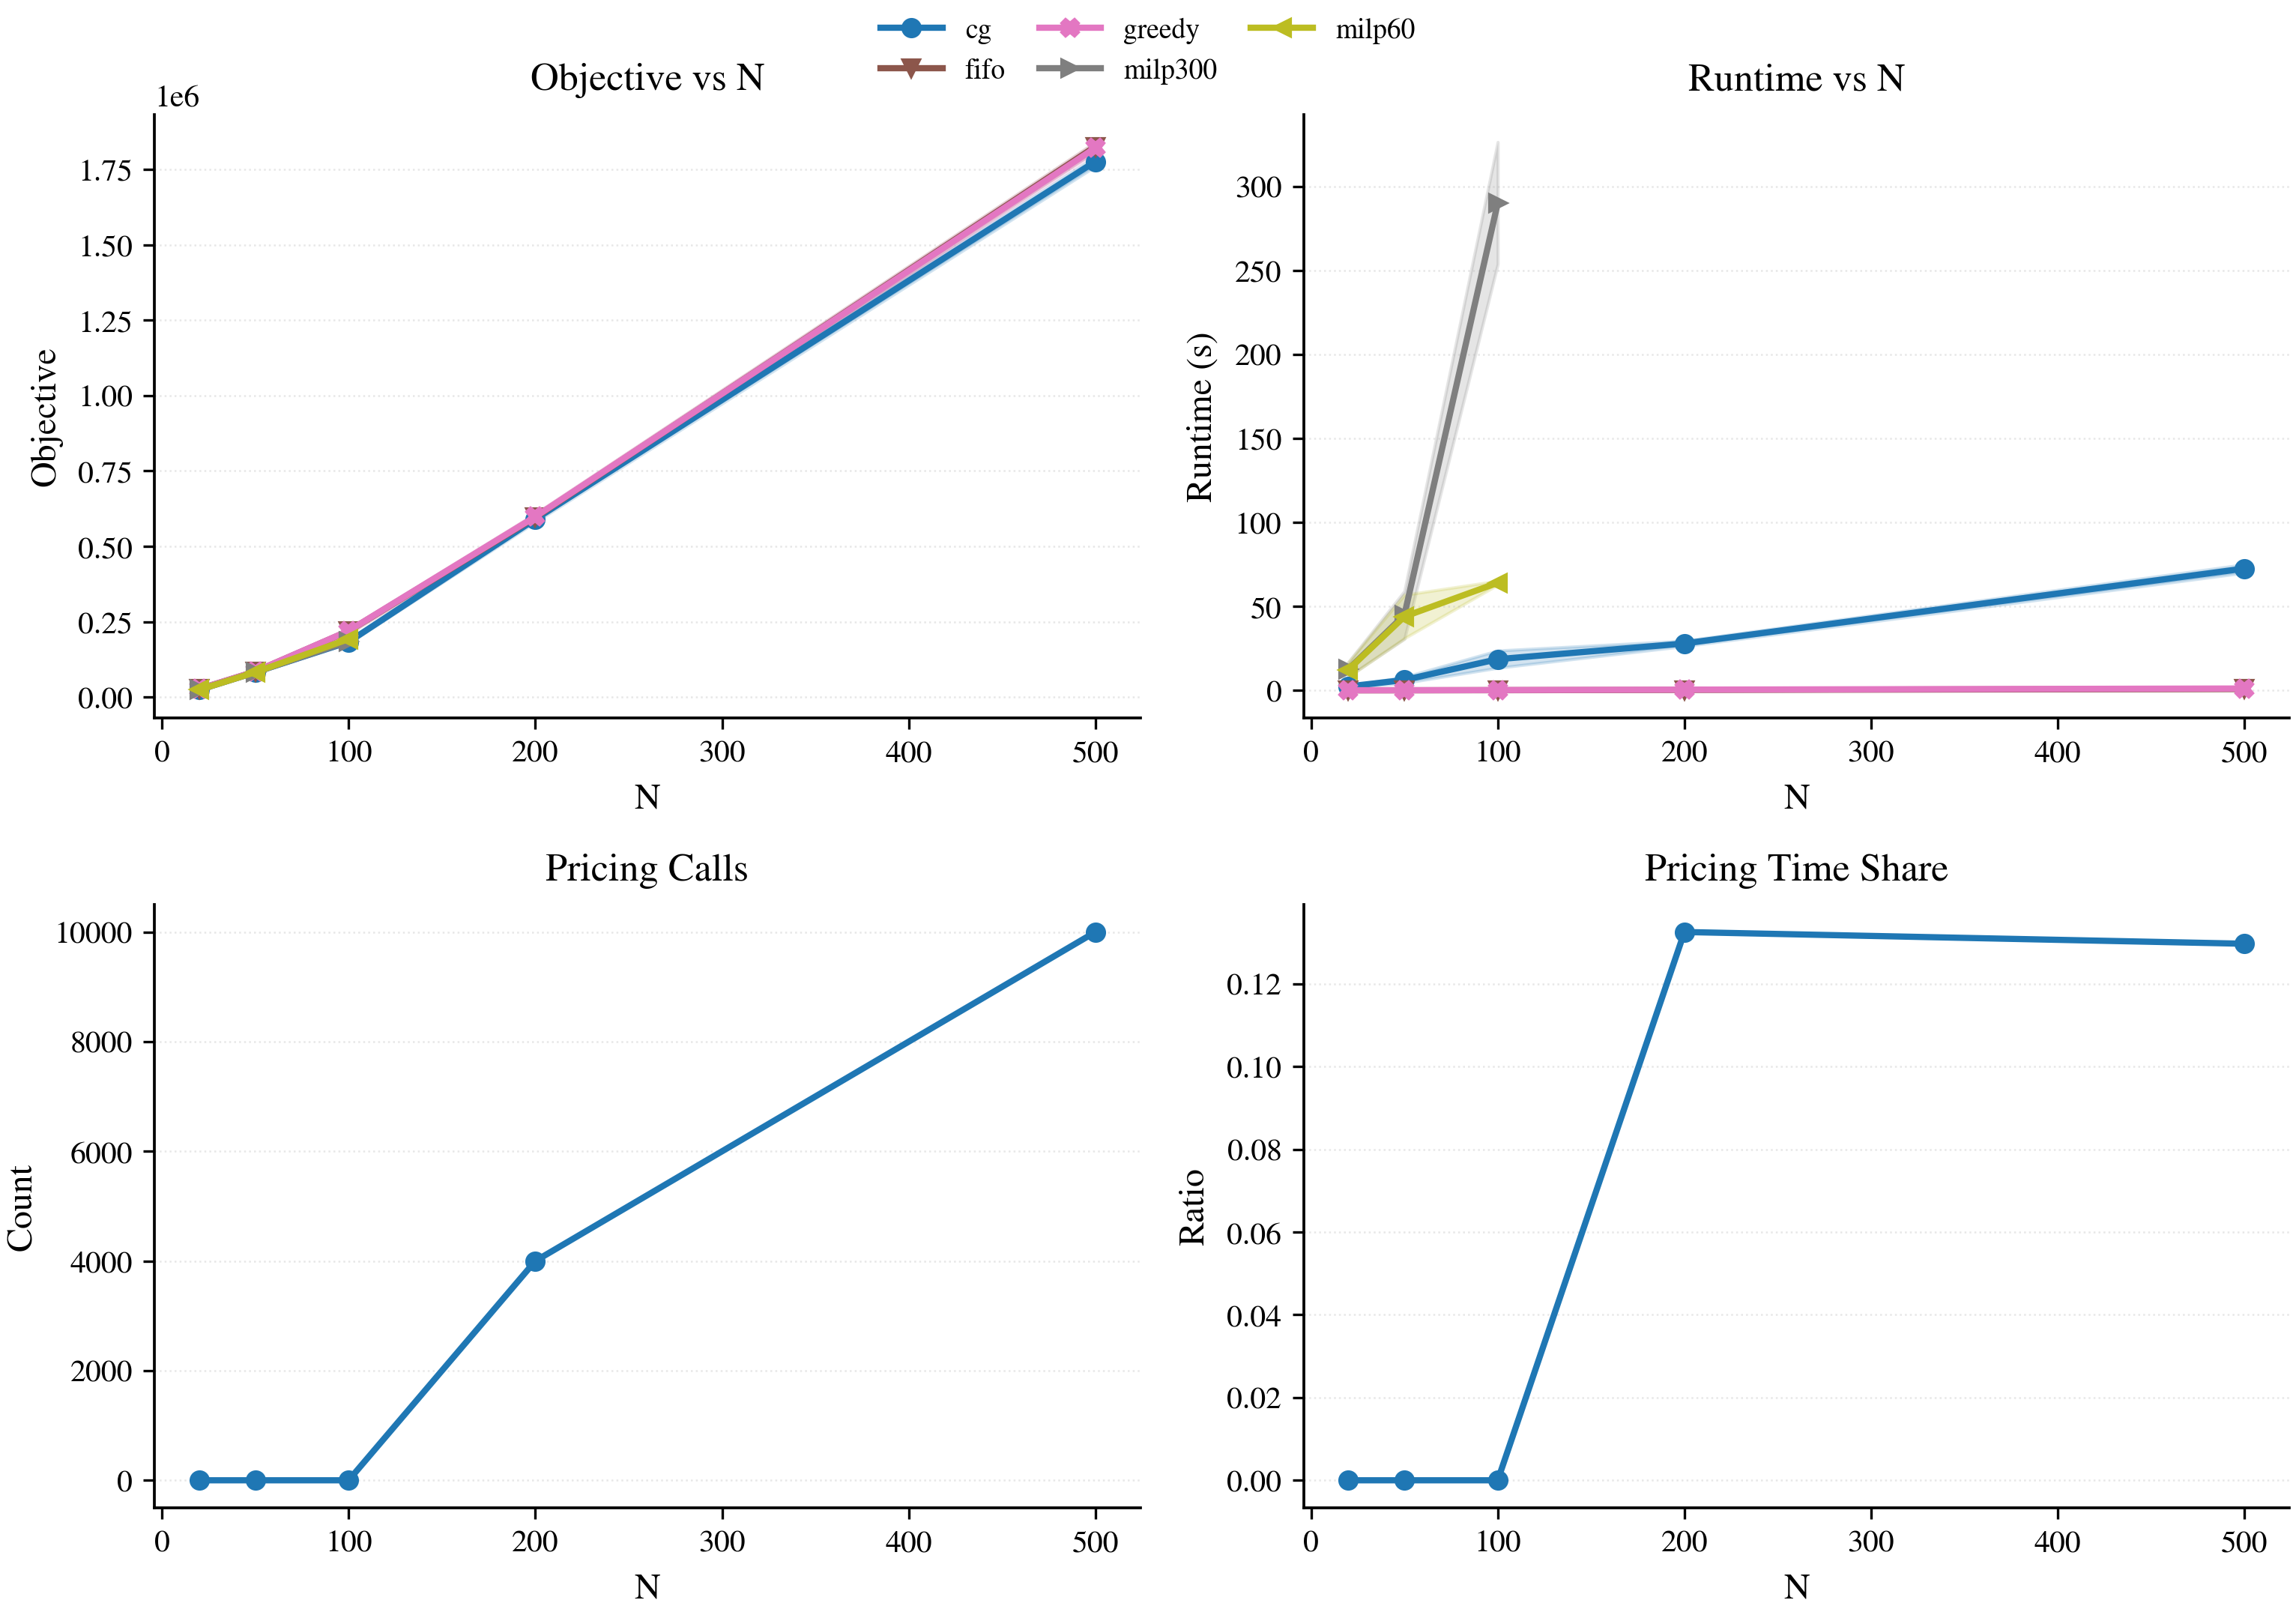
\includegraphics[width=0.95\textwidth]{figs/main/Fig_Main_Combined_U.png}
    \caption{主实验结果：目标值与运行时间随规模变化（U 场景）。}
    \label{fig:main_results}
\end{figure}

\paragraph{场景对比分析}
表 \ref{tab:scenario_results} 与图 \ref{fig:scenario_results} 展示不同到达/服务场景下的表现。峰值到达场景（P）因资源拥堵导致系统成本最高（CG 均值约 186.8k），而长作业场景（L）由于掩盖效应更充分，整体成本最低（约 180.7k）。在三类场景中 CG 均保持最优解质量，运行时间在 L 场景略升高（均值约 58.8s），但仍维持可接受的计算开销。

\begin{table}[htbp]
    \centering
    \caption{场景对比结果（$N=100$）}
    \label{tab:scenario_results}
    \footnotesize
    \begin{tabular}{rlllll}
\toprule
N & scenario & method & obj & runtime & success \\
\midrule
100 & U & CG & 183337.84 $\pm$ 4234.79 & 13.413 $\pm$ 1.632 & 100.0\% \\
100 & U & MILP300 & 184409.83 $\pm$ 5224.13 & 274.707 $\pm$ 41.199 & 40.0\% \\
100 & U & MILP60 & 191850.82 $\pm$ 6475.11 & 62.832 $\pm$ 0.401 & 0.0\% \\
100 & U & Rolling-H & 216035.62 $\pm$ 6299.45 & 119.547 $\pm$ 15.886 & 100.0\% \\
100 & U & F\&O & 205833.37 $\pm$ 6244.45 & 144.821 $\pm$ 28.369 & 100.0\% \\
100 & U & Restricted-CG & 219929.72 $\pm$ 7937.50 & 1.392 $\pm$ 0.222 & 100.0\% \\
100 & U & FIFO & 219354.28 $\pm$ 7613.92 & 0.032 $\pm$ 0.002 & 100.0\% \\
100 & U & Greedy & 220052.50 $\pm$ 7961.84 & 0.070 $\pm$ 0.003 & 100.0\% \\
100 & P & CG & 187028.55 $\pm$ 3070.50 & 16.947 $\pm$ 2.701 & 100.0\% \\
100 & P & MILP300 & 189721.01 $\pm$ 3445.93 & 300.921 $\pm$ 9.350 & 10.0\% \\
100 & P & MILP60 & 198735.34 $\pm$ 2514.18 & 63.704 $\pm$ 0.833 & 0.0\% \\
100 & P & Rolling-H & 228717.35 $\pm$ 4372.44 & 114.180 $\pm$ 14.987 & 100.0\% \\
100 & P & F\&O & 217823.67 $\pm$ 3541.00 & 148.638 $\pm$ 19.718 & 100.0\% \\
100 & P & Restricted-CG & 233177.69 $\pm$ 4843.49 & 1.533 $\pm$ 0.271 & 100.0\% \\
100 & P & FIFO & 231987.03 $\pm$ 5022.10 & 0.068 $\pm$ 0.033 & 100.0\% \\
100 & P & Greedy & 233932.35 $\pm$ 4768.17 & 0.146 $\pm$ 0.063 & 100.0\% \\
100 & L & CG & 181005.36 $\pm$ 4185.47 & 18.126 $\pm$ 4.907 & 100.0\% \\
100 & L & MILP300 & 181038.84 $\pm$ 4195.07 & 272.046 $\pm$ 46.031 & 40.0\% \\
100 & L & MILP60 & 185722.20 $\pm$ 4276.84 & 63.503 $\pm$ 0.992 & 0.0\% \\
100 & L & Rolling-H & 197616.98 $\pm$ 6119.06 & 118.710 $\pm$ 18.332 & 100.0\% \\
100 & L & F\&O & 191604.92 $\pm$ 5141.27 & 144.237 $\pm$ 29.053 & 100.0\% \\
100 & L & Restricted-CG & 203362.74 $\pm$ 6087.35 & 1.635 $\pm$ 0.310 & 100.0\% \\
100 & L & FIFO & 203844.57 $\pm$ 6582.23 & 0.051 $\pm$ 0.031 & 100.0\% \\
100 & L & Greedy & 203452.48 $\pm$ 6117.24 & 0.112 $\pm$ 0.068 & 100.0\% \\
\bottomrule
\end{tabular}

\end{table}

\begin{figure}[htbp]
    \centering
    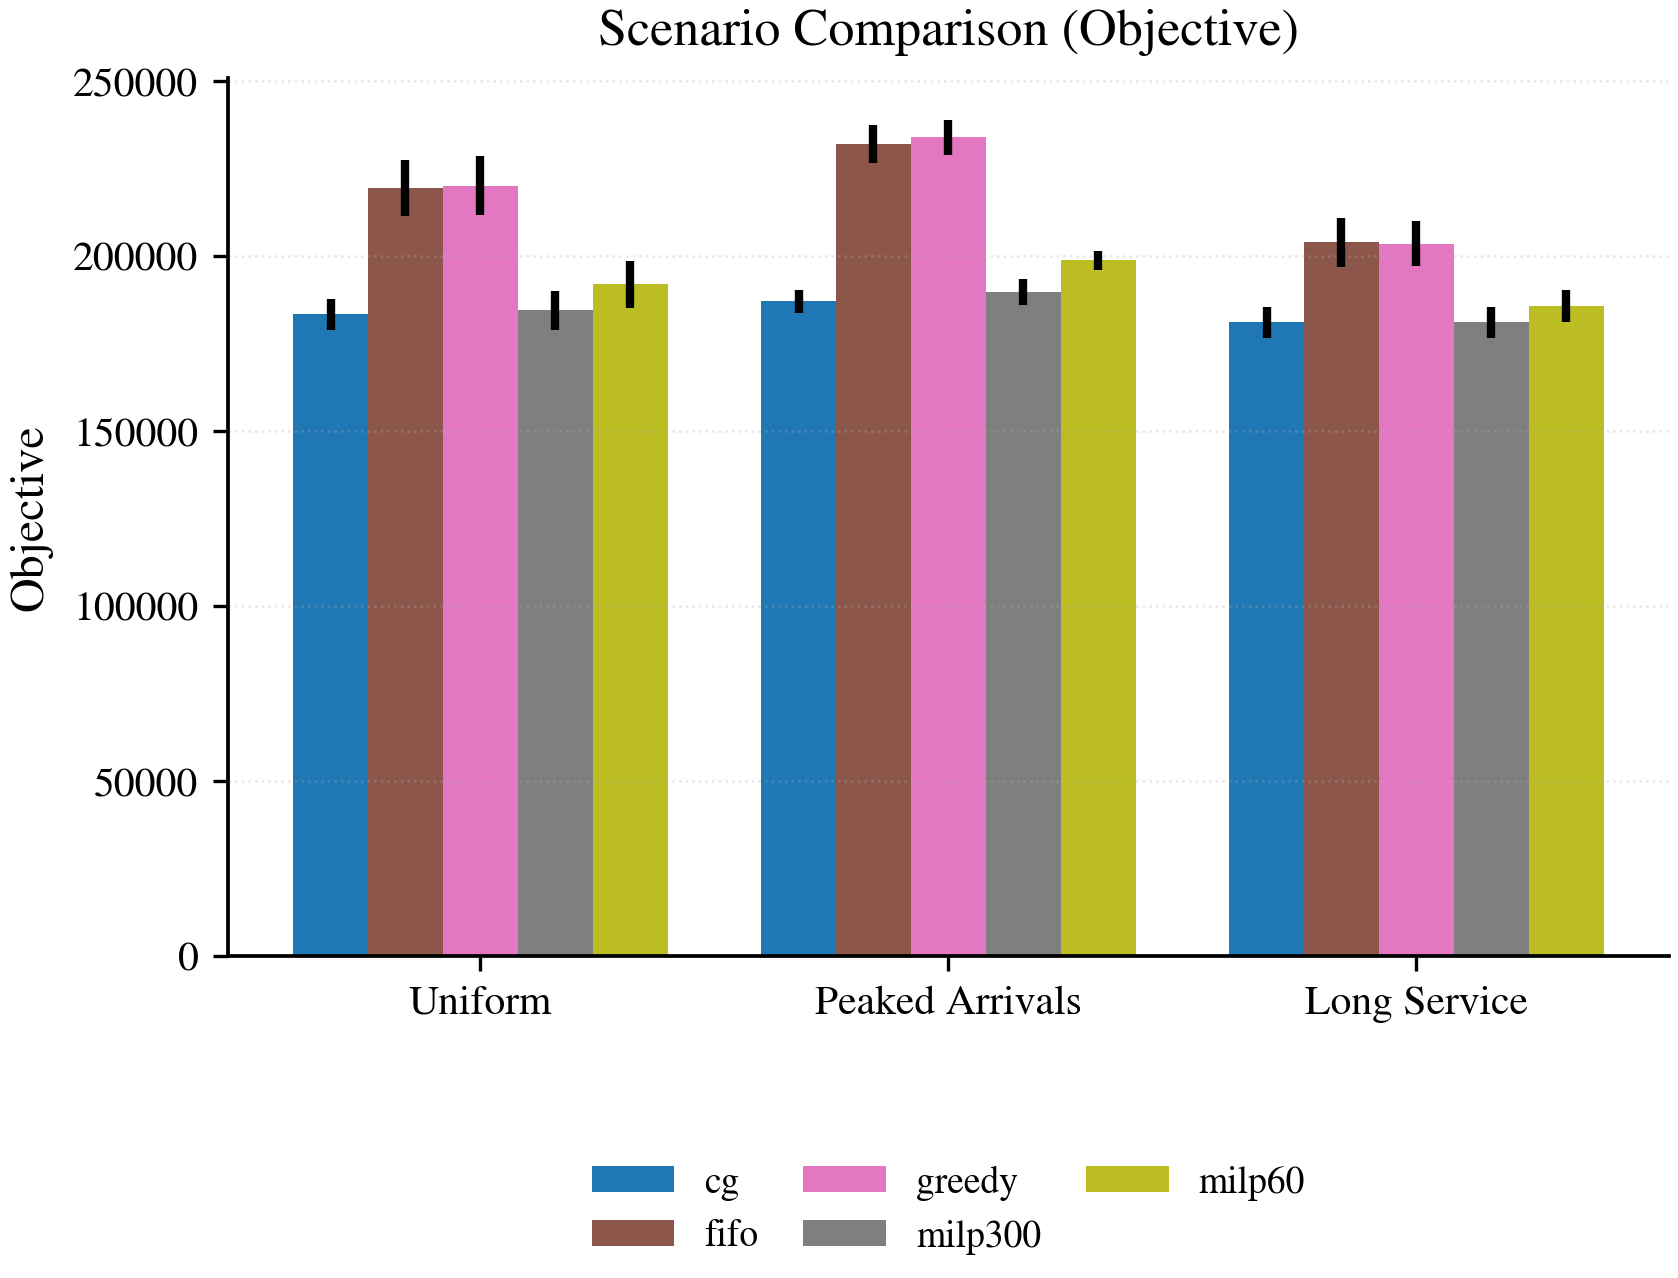
\includegraphics[width=0.85\textwidth]{figs/scenario/Fig_Scenario_Obj.png}
    \caption{不同场景下的目标值对比（$N=100$）。}
    \label{fig:scenario_results}
\end{figure}

\begin{figure}[htbp]
    \centering
    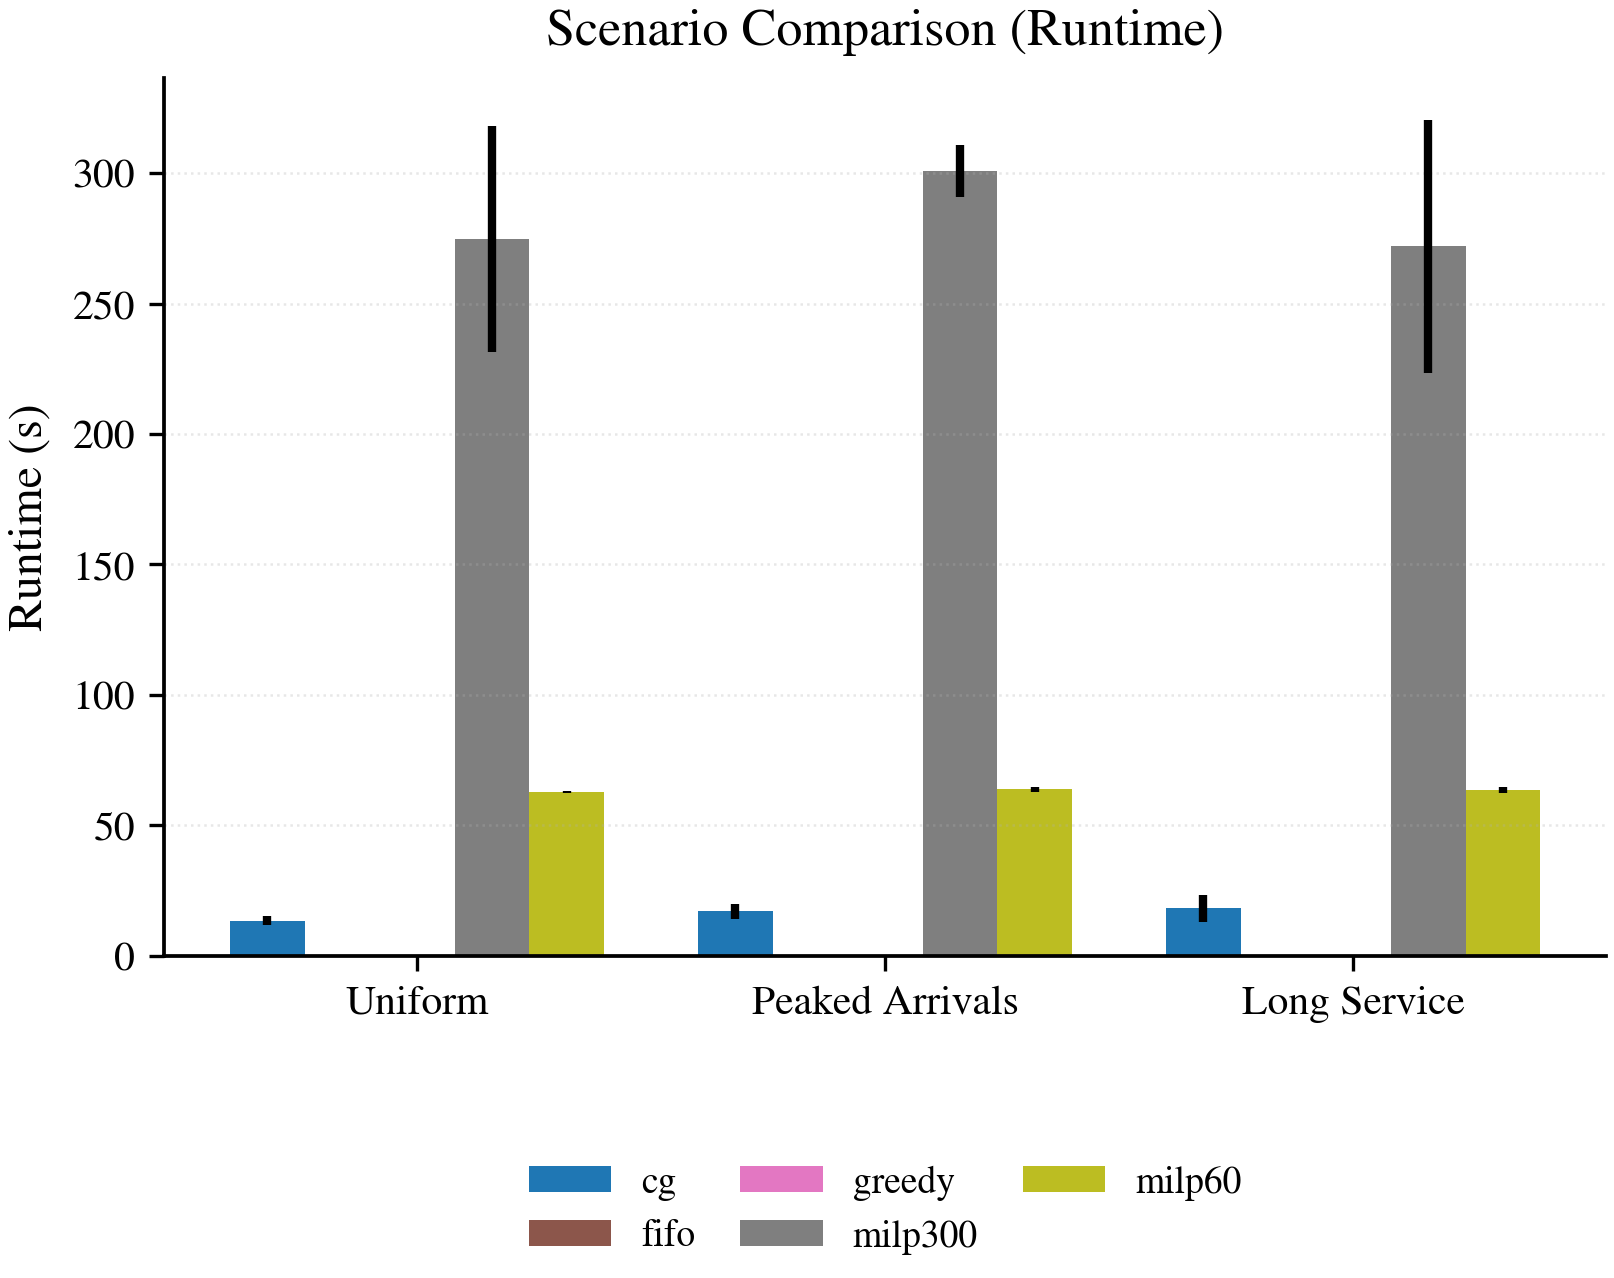
\includegraphics[width=0.85\textwidth]{figs/scenario/Fig_Scenario_Runtime.png}
    \caption{不同场景下的运行时间对比（$N=100$）。}
    \label{fig:scenario_runtime}
\end{figure}

\subsection{SIMOPS 掩盖效应的价值评估}
\label{sec:simops_value}
为量化 SIMOPS 的价值，设置 SIMOPS 与“串行作业”两种操作模式并进行对照实验。表 \ref{tab:simops_results} 与图 \ref{fig:simops_savings} 显示：SIMOPS 在中小规模（$N\le100$）下可显著降低系统成本，而在更大规模（$N\ge200$）下 CG 的优势减弱并出现小幅反转。以 CG 为例，整体平均降本约 9.4\%，在 $N=100$ 时降本约 19.7\%，但在 $N=200/500$ 时分别约为 -0.7\%/-0.8\%。

\begin{table}[htbp]
    \centering
    \caption{SIMOPS 与串行作业对比（均值 $\pm$ 标准差）}
    \label{tab:simops_results}
    \footnotesize
    \begin{tabular}{rlllllll}
\toprule
N & operation_mode & method & obj & runtime & avg_masking_rate & avg_stay_time & success \\
\midrule
25 & sequential & CG & 43206.30 $\pm$ 1438.53 & 1.303 $\pm$ 0.155 & 0.00 $\pm$ 0.00 & 15.98 $\pm$ 0.96 & 100.0\% \\
25 & sequential & Rolling-H & 43694.62 $\pm$ 1695.84 & 16.287 $\pm$ 3.312 & 0.00 $\pm$ 0.00 & 16.20 $\pm$ 0.87 & 100.0\% \\
25 & sequential & F\&O & 43620.62 $\pm$ 1675.96 & 24.489 $\pm$ 8.228 & 0.00 $\pm$ 0.00 & 16.06 $\pm$ 0.84 & 100.0\% \\
25 & sequential & Restricted-CG & 43521.61 $\pm$ 1456.66 & 0.508 $\pm$ 0.076 & 0.00 $\pm$ 0.00 & 15.89 $\pm$ 0.91 & 100.0\% \\
25 & sequential & FIFO & 44650.56 $\pm$ 1426.07 & 0.002 $\pm$ 0.001 & 0.00 $\pm$ 0.00 & 15.81 $\pm$ 0.89 & 100.0\% \\
25 & sequential & Greedy & 44530.56 $\pm$ 1573.87 & 0.017 $\pm$ 0.008 & 0.00 $\pm$ 0.00 & 15.82 $\pm$ 0.89 & 100.0\% \\
25 & simops & CG & 34424.43 $\pm$ 1209.59 & 2.930 $\pm$ 0.728 & 0.80 $\pm$ 0.05 & 14.80 $\pm$ 0.99 & 100.0\% \\
25 & simops & Rolling-H & 35734.72 $\pm$ 1466.13 & 54.104 $\pm$ 17.249 & 0.76 $\pm$ 0.08 & 14.90 $\pm$ 0.95 & 100.0\% \\
25 & simops & F\&O & 35367.48 $\pm$ 1332.51 & 86.696 $\pm$ 23.698 & 0.79 $\pm$ 0.06 & 14.74 $\pm$ 0.82 & 100.0\% \\
25 & simops & Restricted-CG & 36773.63 $\pm$ 1248.27 & 0.617 $\pm$ 0.012 & 0.90 $\pm$ 0.05 & 14.29 $\pm$ 0.79 & 100.0\% \\
25 & simops & FIFO & 37445.33 $\pm$ 1546.82 & 0.008 $\pm$ 0.004 & 0.89 $\pm$ 0.06 & 14.32 $\pm$ 0.77 & 100.0\% \\
25 & simops & Greedy & 36773.63 $\pm$ 1248.27 & 0.036 $\pm$ 0.015 & 0.90 $\pm$ 0.05 & 14.29 $\pm$ 0.79 & 100.0\% \\
50 & sequential & CG & 90235.63 $\pm$ 1853.47 & 2.719 $\pm$ 0.324 & 0.00 $\pm$ 0.00 & 16.65 $\pm$ 0.50 & 100.0\% \\
50 & sequential & Rolling-H & 95805.83 $\pm$ 3647.66 & 26.573 $\pm$ 4.102 & 0.00 $\pm$ 0.00 & 16.54 $\pm$ 0.63 & 100.0\% \\
50 & sequential & F\&O & 95714.58 $\pm$ 3393.67 & 34.988 $\pm$ 6.321 & 0.00 $\pm$ 0.00 & 16.28 $\pm$ 0.55 & 100.0\% \\
50 & sequential & Restricted-CG & 92250.47 $\pm$ 1913.42 & 0.655 $\pm$ 0.014 & 0.00 $\pm$ 0.00 & 16.34 $\pm$ 0.50 & 100.0\% \\
50 & sequential & FIFO & 98608.17 $\pm$ 4748.70 & 0.010 $\pm$ 0.004 & 0.00 $\pm$ 0.00 & 15.97 $\pm$ 0.53 & 100.0\% \\
50 & sequential & Greedy & 98267.16 $\pm$ 4827.22 & 0.046 $\pm$ 0.017 & 0.00 $\pm$ 0.00 & 16.05 $\pm$ 0.53 & 100.0\% \\
50 & simops & CG & 82695.01 $\pm$ 2369.33 & 8.376 $\pm$ 2.272 & 0.82 $\pm$ 0.05 & 15.06 $\pm$ 0.45 & 100.0\% \\
50 & simops & Rolling-H & 85160.42 $\pm$ 2990.49 & 87.224 $\pm$ 23.003 & 0.79 $\pm$ 0.05 & 15.16 $\pm$ 0.47 & 100.0\% \\
50 & simops & F\&O & 83757.48 $\pm$ 2381.76 & 102.192 $\pm$ 37.531 & 0.87 $\pm$ 0.05 & 14.88 $\pm$ 0.53 & 100.0\% \\
50 & simops & Restricted-CG & 85168.31 $\pm$ 3065.64 & 0.832 $\pm$ 0.055 & 0.92 $\pm$ 0.02 & 14.73 $\pm$ 0.55 & 100.0\% \\
50 & simops & FIFO & 85133.55 $\pm$ 2627.06 & 0.034 $\pm$ 0.003 & 0.90 $\pm$ 0.02 & 14.82 $\pm$ 0.47 & 100.0\% \\
50 & simops & Greedy & 85168.31 $\pm$ 3065.64 & 0.103 $\pm$ 0.007 & 0.92 $\pm$ 0.02 & 14.73 $\pm$ 0.55 & 100.0\% \\
100 & sequential & CG & 228619.37 $\pm$ 10518.33 & 6.072 $\pm$ 0.777 & 0.00 $\pm$ 0.00 & 13.51 $\pm$ 0.78 & 100.0\% \\
100 & sequential & Rolling-H & 262461.98 $\pm$ 10915.47 & 44.357 $\pm$ 5.406 & 0.00 $\pm$ 0.00 & 12.45 $\pm$ 0.57 & 100.0\% \\
100 & sequential & F\&O & 259702.83 $\pm$ 11653.10 & 61.445 $\pm$ 4.707 & 0.00 $\pm$ 0.00 & 12.60 $\pm$ 0.58 & 100.0\% \\
100 & sequential & Restricted-CG & 238942.94 $\pm$ 8948.64 & 0.960 $\pm$ 0.046 & 0.00 $\pm$ 0.00 & 12.53 $\pm$ 0.54 & 100.0\% \\
100 & sequential & FIFO & 268483.17 $\pm$ 11391.13 & 0.039 $\pm$ 0.005 & 0.00 $\pm$ 0.00 & 12.39 $\pm$ 0.57 & 100.0\% \\
100 & sequential & Greedy & 268621.18 $\pm$ 11183.05 & 0.129 $\pm$ 0.017 & 0.00 $\pm$ 0.00 & 12.27 $\pm$ 0.58 & 100.0\% \\
100 & simops & CG & 183338.23 $\pm$ 4235.48 & 36.425 $\pm$ 22.378 & 0.49 $\pm$ 0.04 & 15.98 $\pm$ 0.30 & 100.0\% \\
100 & simops & Rolling-H & 215943.91 $\pm$ 6157.53 & 117.675 $\pm$ 20.367 & 0.46 $\pm$ 0.03 & 15.63 $\pm$ 0.43 & 100.0\% \\
100 & simops & F\&O & 205833.37 $\pm$ 6244.45 & 140.984 $\pm$ 26.734 & 0.52 $\pm$ 0.04 & 15.54 $\pm$ 0.36 & 100.0\% \\
100 & simops & Restricted-CG & 219929.72 $\pm$ 7937.50 & 1.263 $\pm$ 0.066 & 0.60 $\pm$ 0.03 & 15.15 $\pm$ 0.29 & 100.0\% \\
100 & simops & FIFO & 219354.28 $\pm$ 7613.92 & 0.105 $\pm$ 0.019 & 0.60 $\pm$ 0.03 & 15.16 $\pm$ 0.31 & 100.0\% \\
100 & simops & Greedy & 220052.50 $\pm$ 7961.84 & 0.213 $\pm$ 0.040 & 0.60 $\pm$ 0.03 & 15.14 $\pm$ 0.29 & 100.0\% \\
200 & sequential & CG & 587846.64 $\pm$ 7877.12 & 8.781 $\pm$ 2.504 & 0.00 $\pm$ 0.00 & 7.62 $\pm$ 0.23 & 100.0\% \\
200 & sequential & Rolling-H & 653442.35 $\pm$ 12920.52 & 81.240 $\pm$ 7.926 & 0.00 $\pm$ 0.00 & 7.83 $\pm$ 0.30 & 100.0\% \\
200 & sequential & F\&O & 648171.73 $\pm$ 11894.11 & 112.033 $\pm$ 4.923 & 0.00 $\pm$ 0.00 & 7.88 $\pm$ 0.32 & 100.0\% \\
200 & sequential & Restricted-CG & 599890.78 $\pm$ 8178.84 & 1.790 $\pm$ 0.308 & 0.00 $\pm$ 0.00 & 7.58 $\pm$ 0.30 & 100.0\% \\
200 & sequential & FIFO & 659122.58 $\pm$ 12265.67 & 0.113 $\pm$ 0.007 & 0.00 $\pm$ 0.00 & 7.89 $\pm$ 0.30 & 100.0\% \\
200 & sequential & Greedy & 658255.39 $\pm$ 12640.22 & 0.216 $\pm$ 0.061 & 0.00 $\pm$ 0.00 & 7.87 $\pm$ 0.34 & 100.0\% \\
200 & simops & CG & 535891.97 $\pm$ 7703.35 & 102.797 $\pm$ 20.068 & 0.27 $\pm$ 0.02 & 15.01 $\pm$ 0.35 & 100.0\% \\
200 & simops & Rolling-H & 600494.56 $\pm$ 9041.30 & 182.366 $\pm$ 16.138 & 0.20 $\pm$ 0.02 & 15.10 $\pm$ 0.37 & 100.0\% \\
200 & simops & F\&O & 584333.63 $\pm$ 10604.41 & 215.477 $\pm$ 16.309 & 0.26 $\pm$ 0.02 & 14.98 $\pm$ 0.36 & 100.0\% \\
200 & simops & Restricted-CG & 598148.62 $\pm$ 9973.23 & 2.551 $\pm$ 0.481 & 0.27 $\pm$ 0.02 & 14.99 $\pm$ 0.37 & 100.0\% \\
200 & simops & FIFO & 596409.36 $\pm$ 10226.59 & 0.255 $\pm$ 0.018 & 0.27 $\pm$ 0.02 & 15.01 $\pm$ 0.35 & 100.0\% \\
200 & simops & Greedy & 598402.66 $\pm$ 9889.80 & 0.408 $\pm$ 0.036 & 0.27 $\pm$ 0.02 & 15.00 $\pm$ 0.37 & 100.0\% \\
500 & sequential & CG & 1760133.70 $\pm$ 15888.91 & 17.366 $\pm$ 3.782 & 0.00 $\pm$ 0.00 & 3.45 $\pm$ 0.10 & 100.0\% \\
500 & sequential & Rolling-H & 1876084.68 $\pm$ 13107.67 & 163.584 $\pm$ 5.346 & 0.00 $\pm$ 0.00 & 3.83 $\pm$ 0.09 & 100.0\% \\
500 & sequential & F\&O & 1873453.21 $\pm$ 14291.36 & 235.541 $\pm$ 14.509 & 0.00 $\pm$ 0.00 & 3.84 $\pm$ 0.10 & 100.0\% \\
500 & sequential & Restricted-CG & 1774700.37 $\pm$ 15342.83 & 2.906 $\pm$ 0.107 & 0.00 $\pm$ 0.00 & 3.50 $\pm$ 0.09 & 100.0\% \\
500 & sequential & FIFO & 1884659.29 $\pm$ 13316.98 & 0.335 $\pm$ 0.078 & 0.00 $\pm$ 0.00 & 3.87 $\pm$ 0.10 & 100.0\% \\
500 & sequential & Greedy & 1881270.19 $\pm$ 15802.41 & 0.611 $\pm$ 0.135 & 0.00 $\pm$ 0.00 & 3.85 $\pm$ 0.09 & 100.0\% \\
500 & simops & CG & 1690831.88 $\pm$ 13429.77 & 238.076 $\pm$ 10.500 & 0.11 $\pm$ 0.01 & 14.55 $\pm$ 0.21 & 100.0\% \\
500 & simops & Rolling-H & 1827529.27 $\pm$ 13567.55 & 327.121 $\pm$ 24.439 & 0.08 $\pm$ 0.00 & 14.73 $\pm$ 0.19 & 100.0\% \\
500 & simops & F\&O & 1810142.23 $\pm$ 14619.54 & 401.871 $\pm$ 28.877 & 0.10 $\pm$ 0.01 & 14.69 $\pm$ 0.21 & 100.0\% \\
500 & simops & Restricted-CG & 1821088.59 $\pm$ 15552.70 & 4.996 $\pm$ 0.151 & 0.10 $\pm$ 0.01 & 14.70 $\pm$ 0.21 & 100.0\% \\
500 & simops & FIFO & 1825679.25 $\pm$ 14168.46 & 0.773 $\pm$ 0.026 & 0.10 $\pm$ 0.01 & 14.74 $\pm$ 0.20 & 100.0\% \\
500 & simops & Greedy & 1821269.84 $\pm$ 15666.30 & 1.082 $\pm$ 0.051 & 0.10 $\pm$ 0.01 & 14.70 $\pm$ 0.21 & 100.0\% \\
\bottomrule
\end{tabular}

\end{table}

\begin{figure}[htbp]
    \centering
    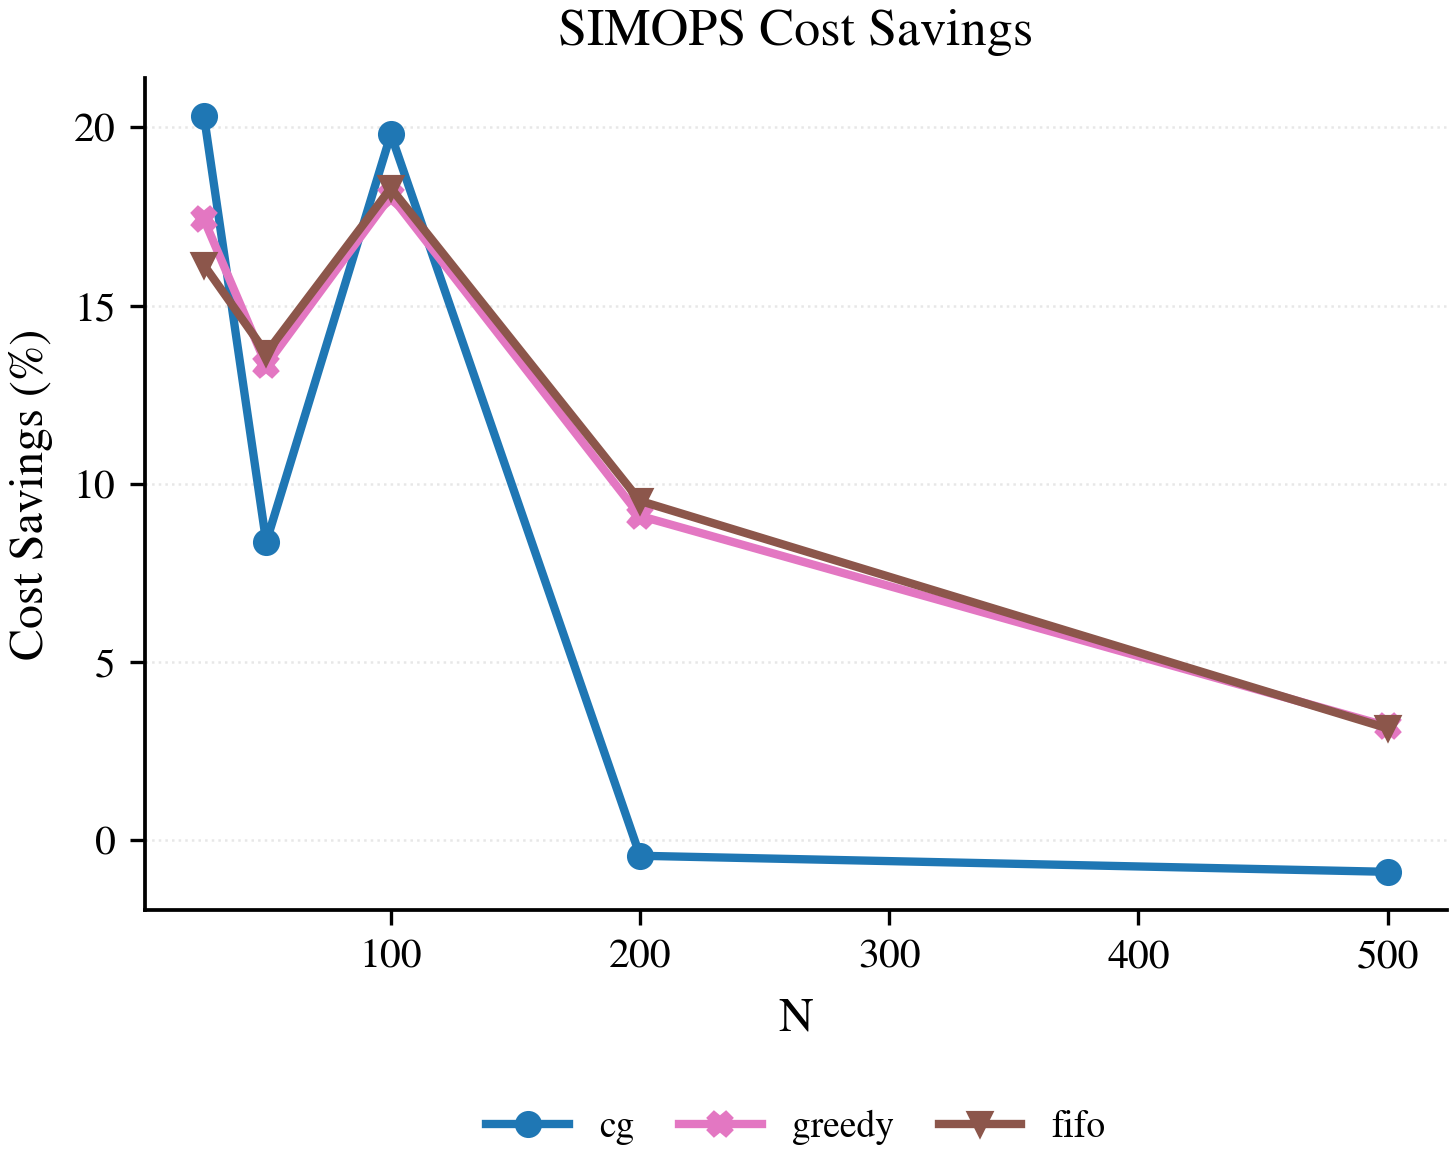
\includegraphics[width=0.85\textwidth]{figs/simops/Fig_SIMOPS_Cost_Savings.png}
    \caption{SIMOPS 相对于串行作业的成本节约比例。}
    \label{fig:simops_savings}
\end{figure}

图 \ref{fig:masking_dist} 给出了 SIMOPS 掩盖率分布，平均掩盖率约为 0.51（CG），范围约为 $[0.12,0.90]$，说明该效应在不同实例中普遍存在但强度不同。按船舶类型拆分（图 \ref{fig:masking_type}），高时敏类型 A 的掩盖收益最大，类型 D 最低（类型 C 次低），体现了资源兼容性与掩盖效应的耦合关系。图 \ref{fig:gantt_simops} 进一步从单实例角度展示了 SIMOPS 下能源服务与装卸作业的时间重叠，从而减少实际离港延误。

\begin{figure}[htbp]
    \centering
    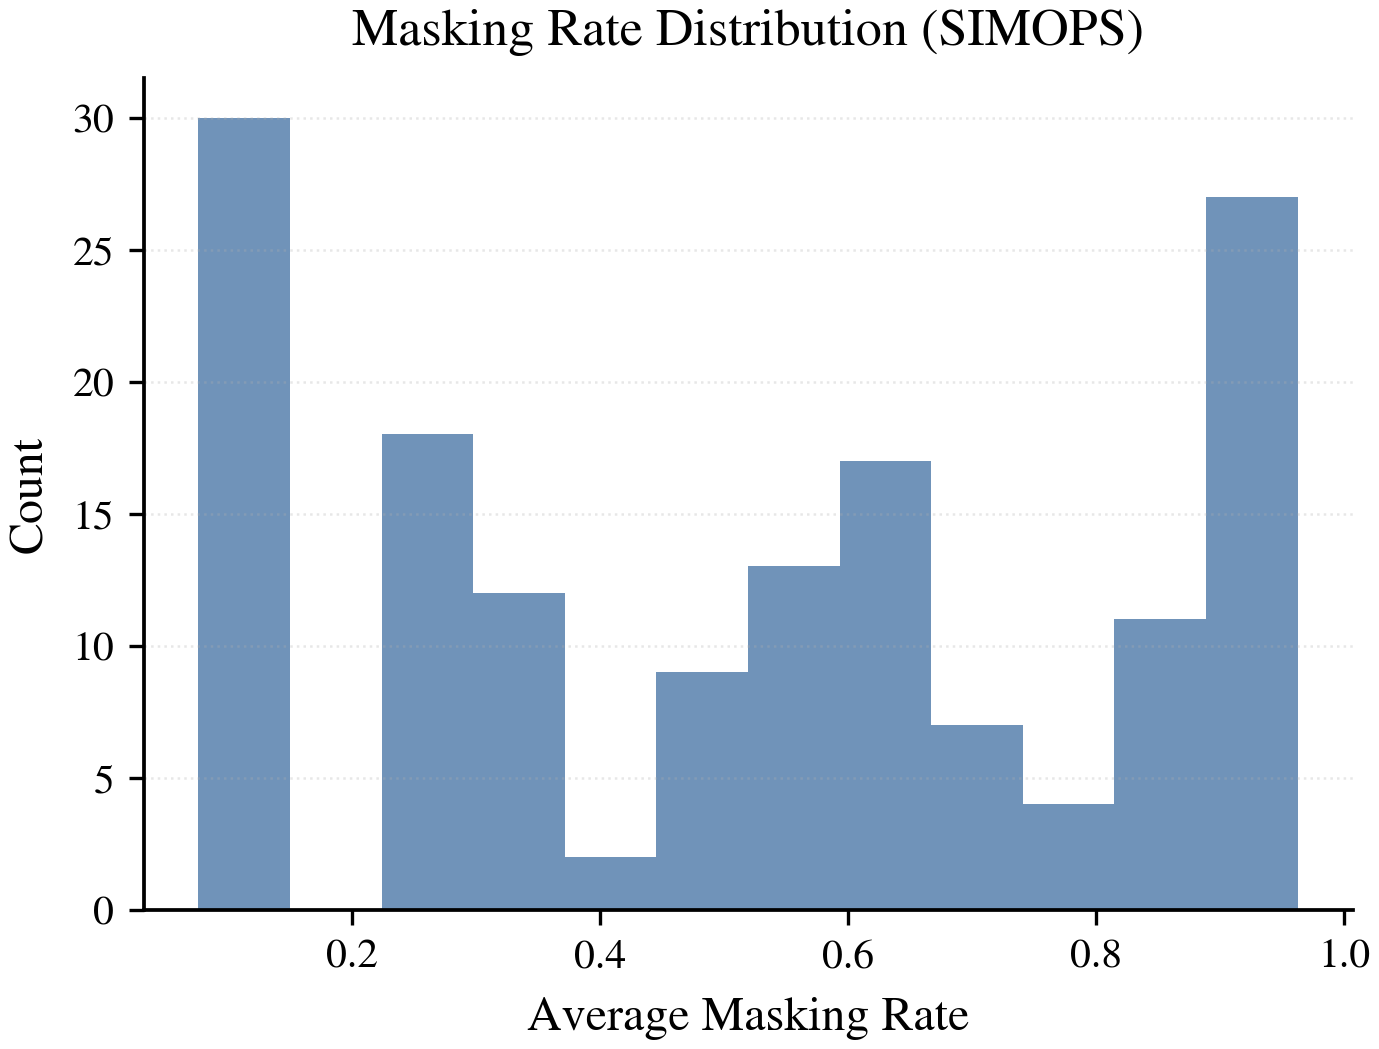
\includegraphics[width=0.85\textwidth]{figs/simops/Fig_SIMOPS_Masking_Distribution.png}
    \caption{SIMOPS 掩盖率分布（CG）。}
    \label{fig:masking_dist}
\end{figure}

\begin{figure}[htbp]
    \centering
    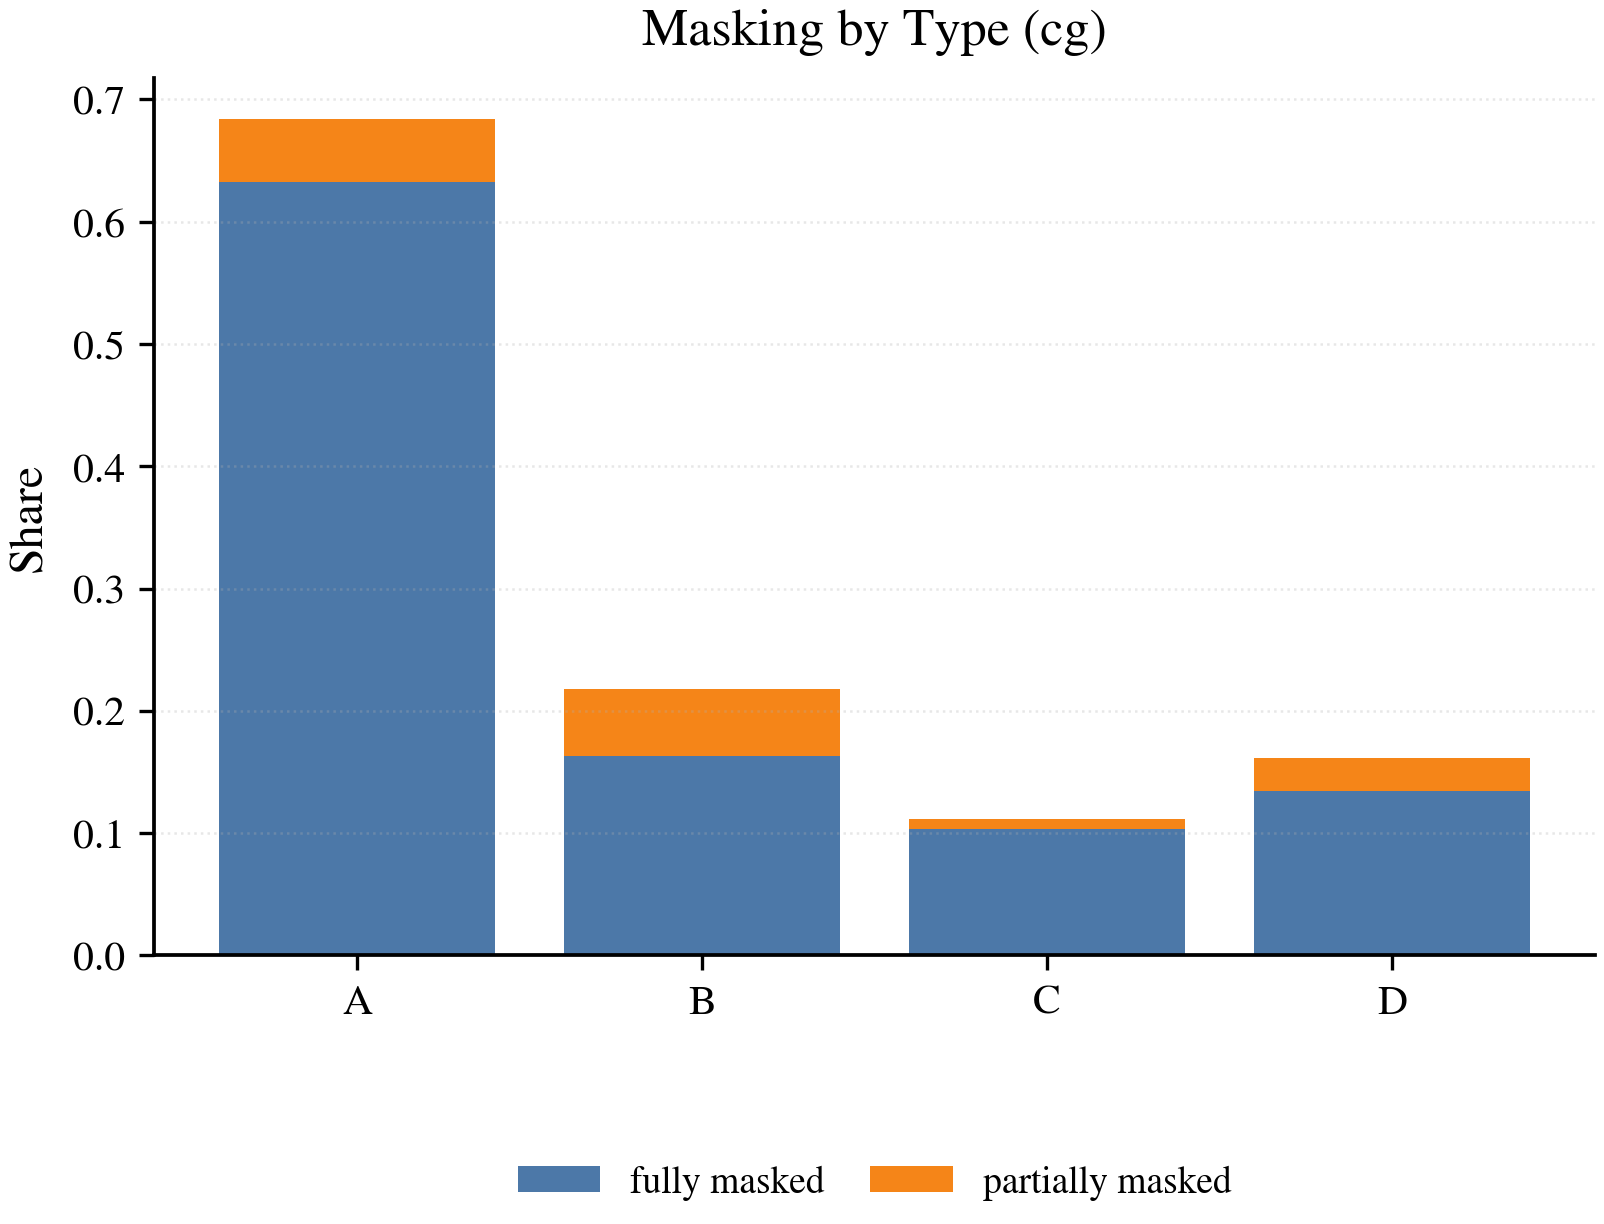
\includegraphics[width=0.85\textwidth]{figs/simops/Fig_SIMOPS_Masking_By_Type.png}
    \caption{不同船舶类型的掩盖效果（CG）。}
    \label{fig:masking_type}
\end{figure}

\begin{figure}[htbp]
    \centering
    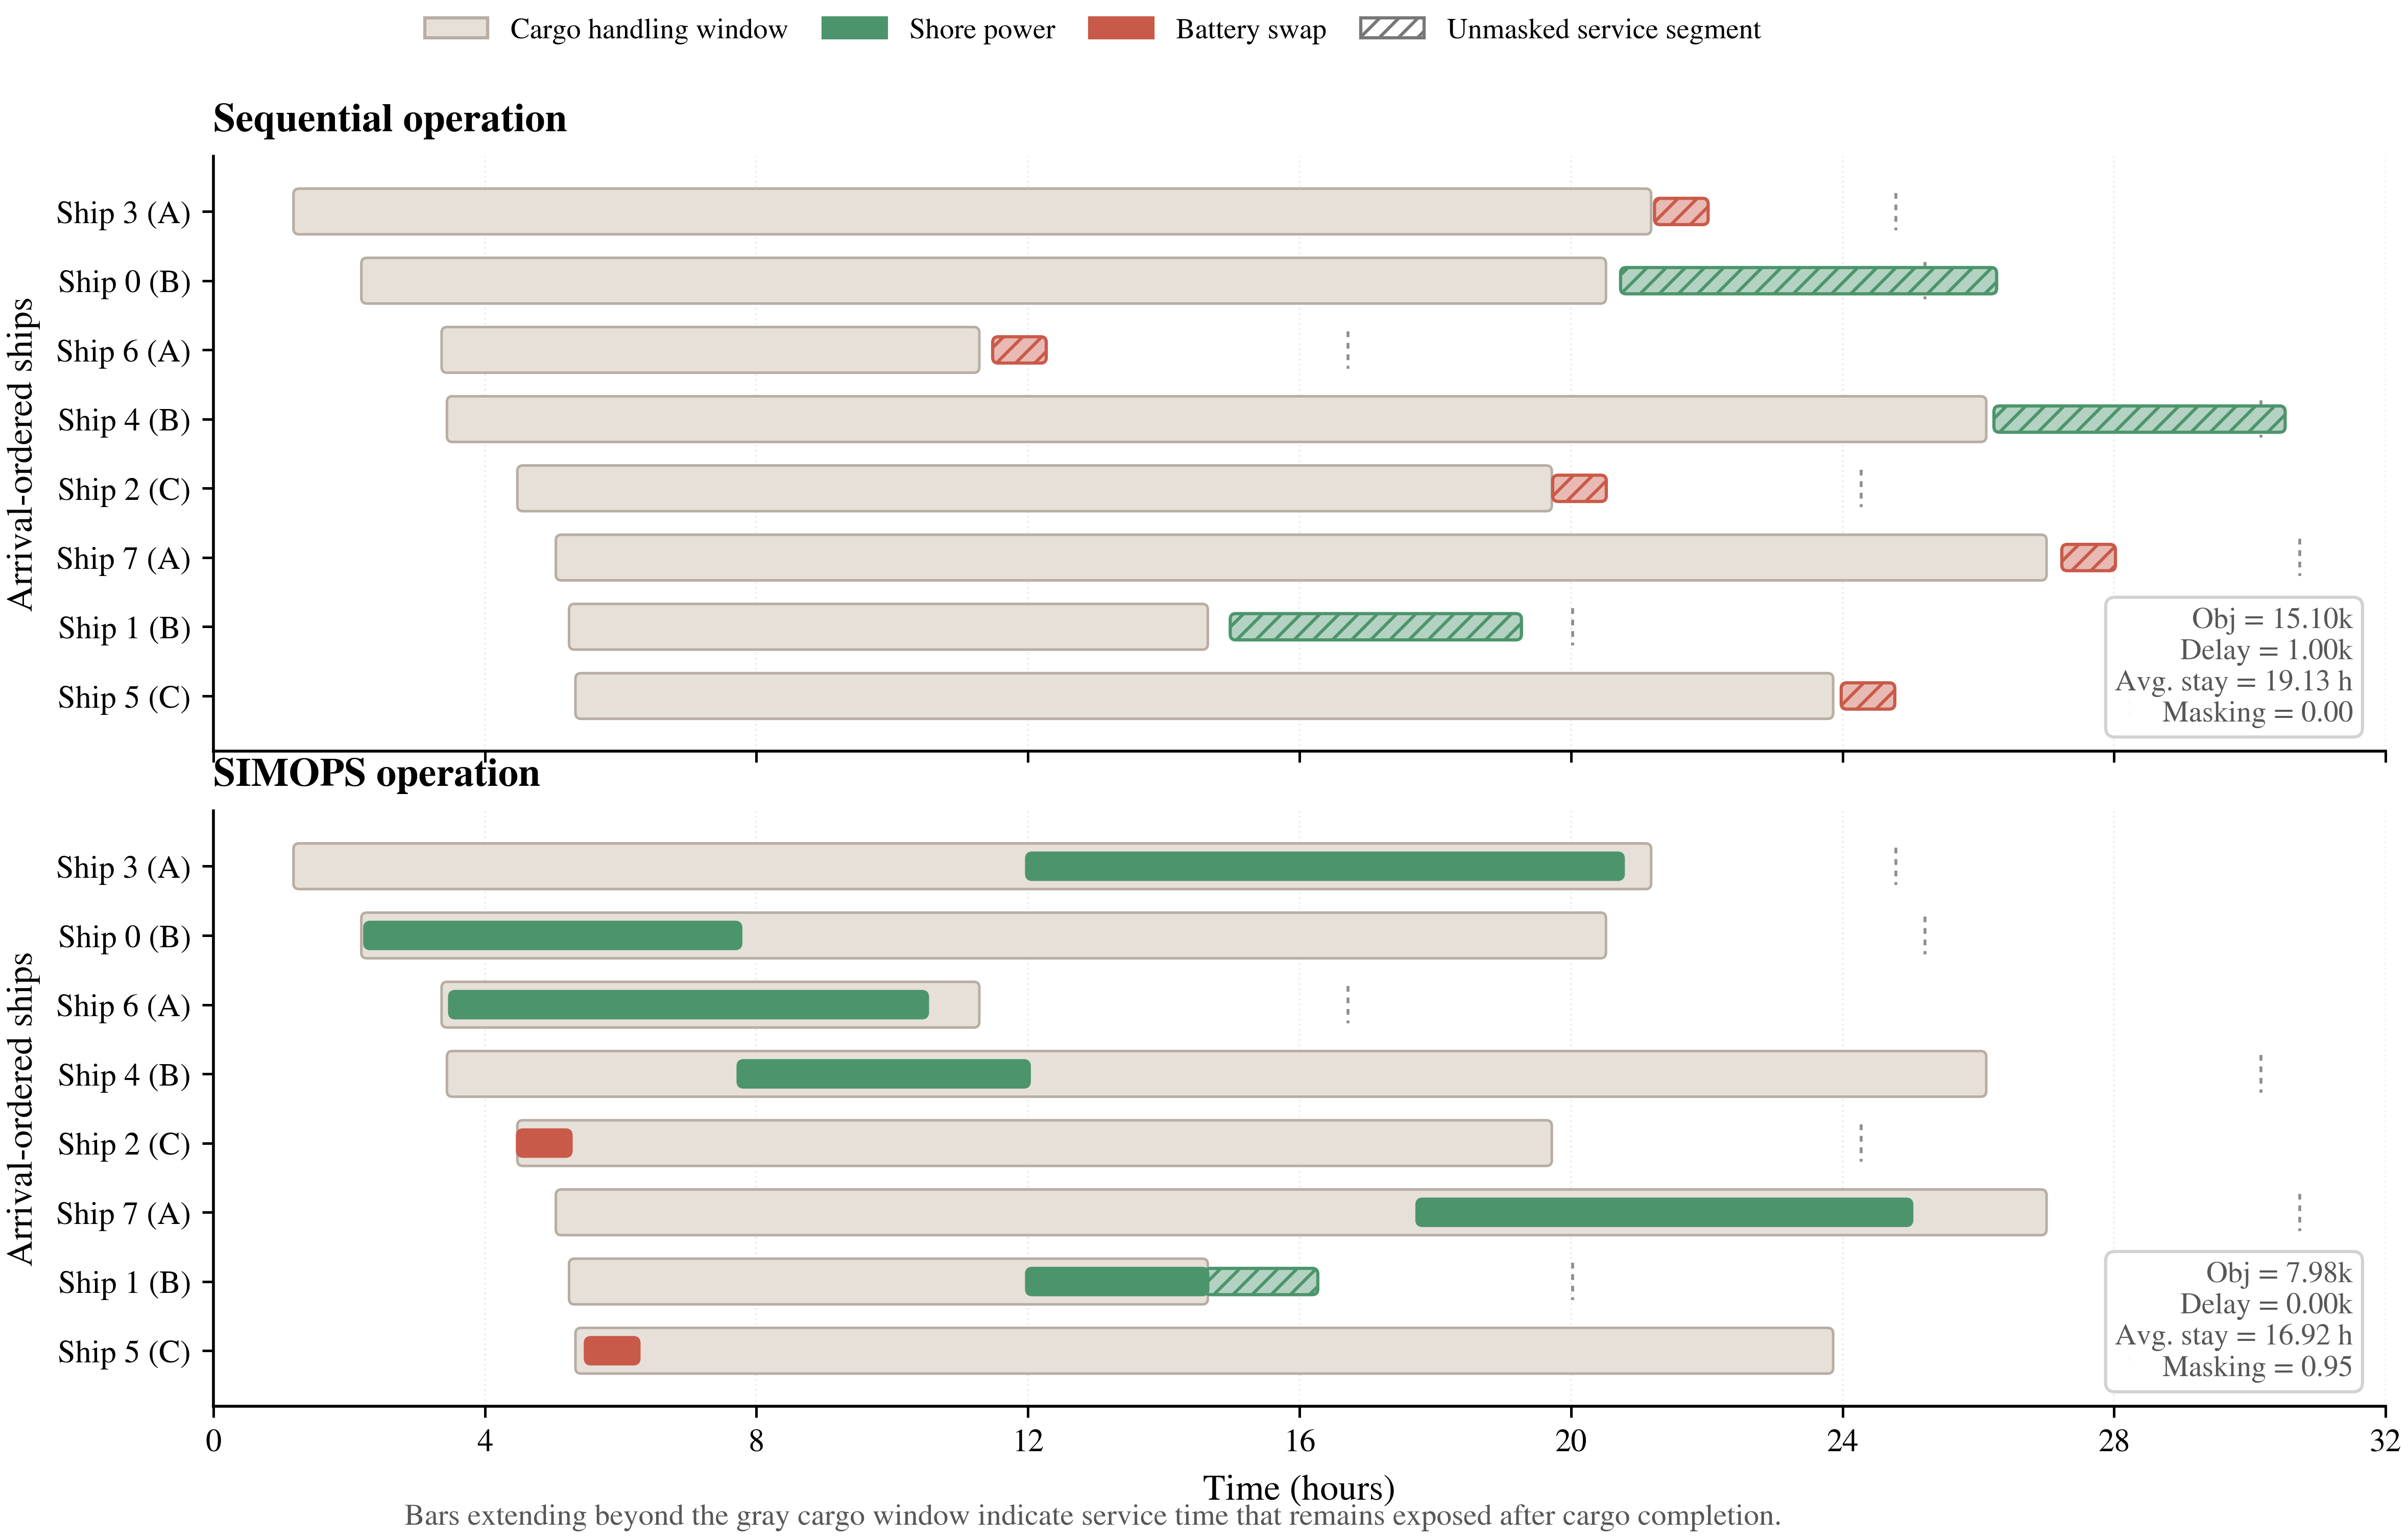
\includegraphics[width=0.95\textwidth]{figs/simops/Fig_SIMOPS_Gantt_Comparison.png}
    \caption{SIMOPS 与串行作业的甘特示例对比。}
    \label{fig:gantt_simops}
\end{figure}

\subsection{敏感性分析与管理启示}
\label{sec:sensitivity}
图 \ref{fig:sens_battery}--\ref{fig:sens_deadline} 总结了关键参数的敏感性结果（$N=100$，U 场景）。电池成本由 0.30 增至 0.80 \$/kWh 时，系统总成本均值由约 125k 上升至 319k，电池占比略降、褐色占比小幅上升。岸电桩数量由 1 增至 8 时，总成本由约 198k 降至 133k，同时褐色占比由 0.032 降至 0，说明岸电基础设施扩容对系统成本与绿色占比具有显著改善作用。紧迫度系数从 0.8 提升至 1.2 时，系统成本约下降 1.3\%，褐色占比同步下降，反映出更充裕的时间窗口有助于提升绿色能源使用比例。

\begin{figure}[htbp]
    \centering
    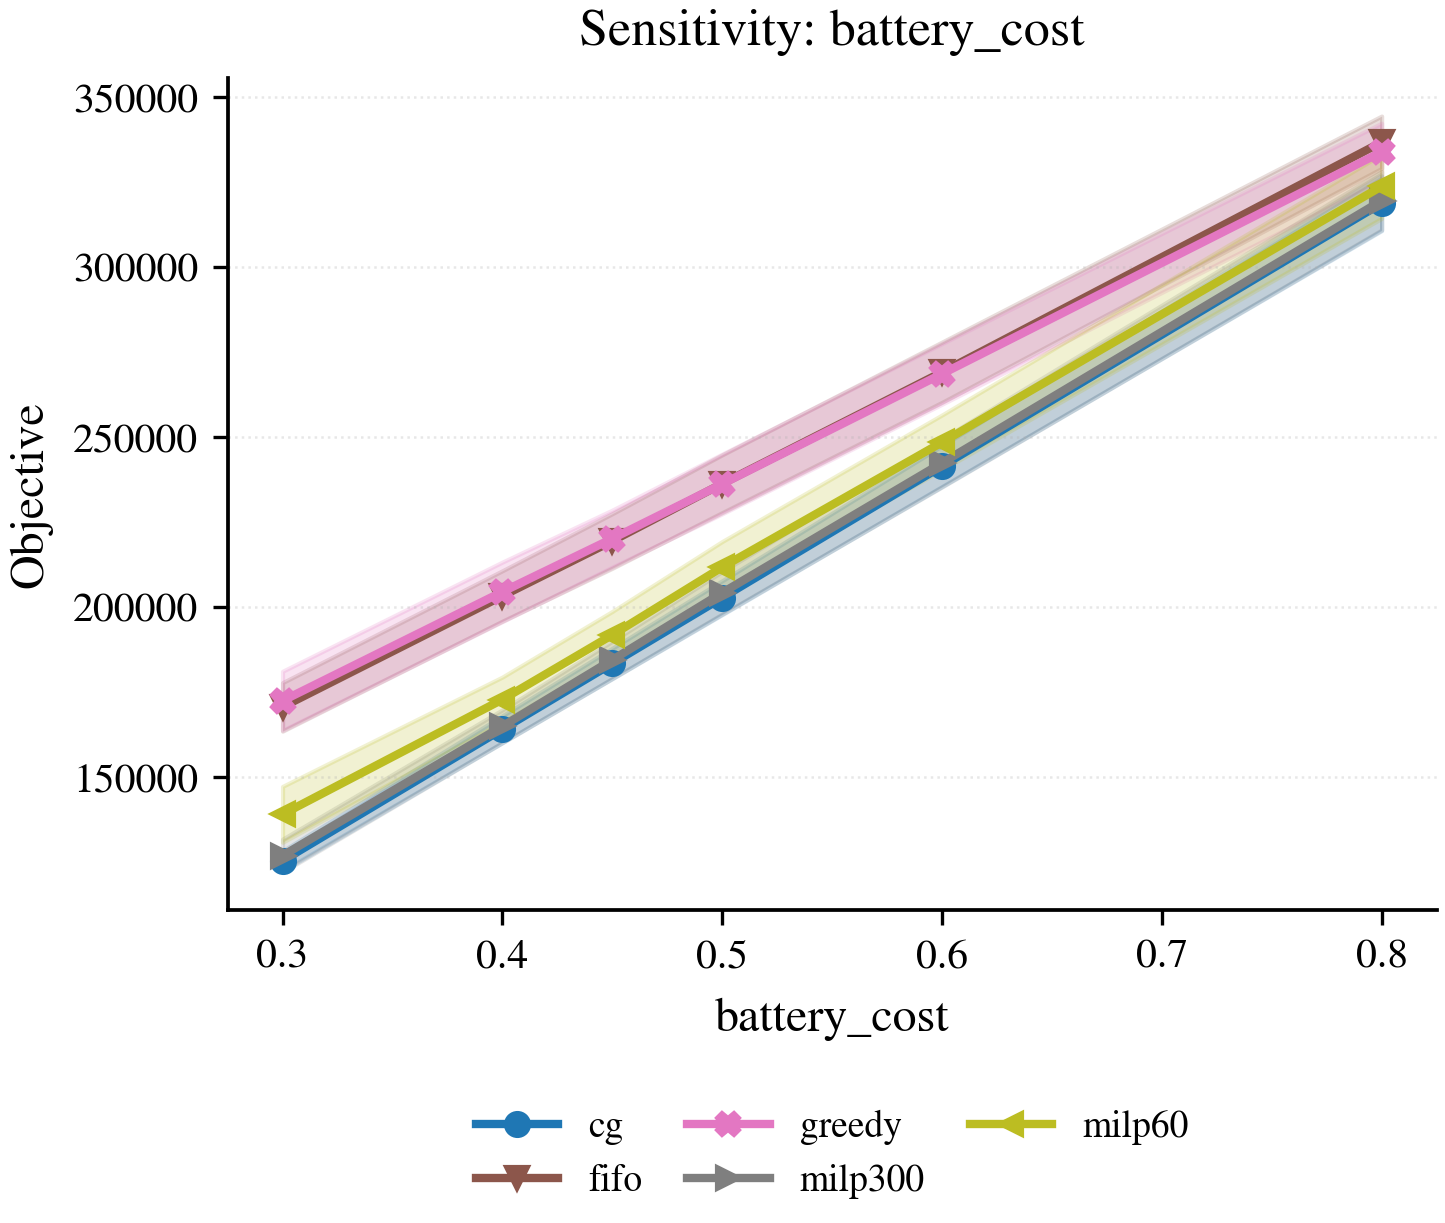
\includegraphics[width=0.85\textwidth]{figs/sensitivity/Fig_Sens_BatteryCost.png}
    \caption{电池成本敏感性分析（CG）。}
    \label{fig:sens_battery}
\end{figure}

\begin{figure}[htbp]
    \centering
    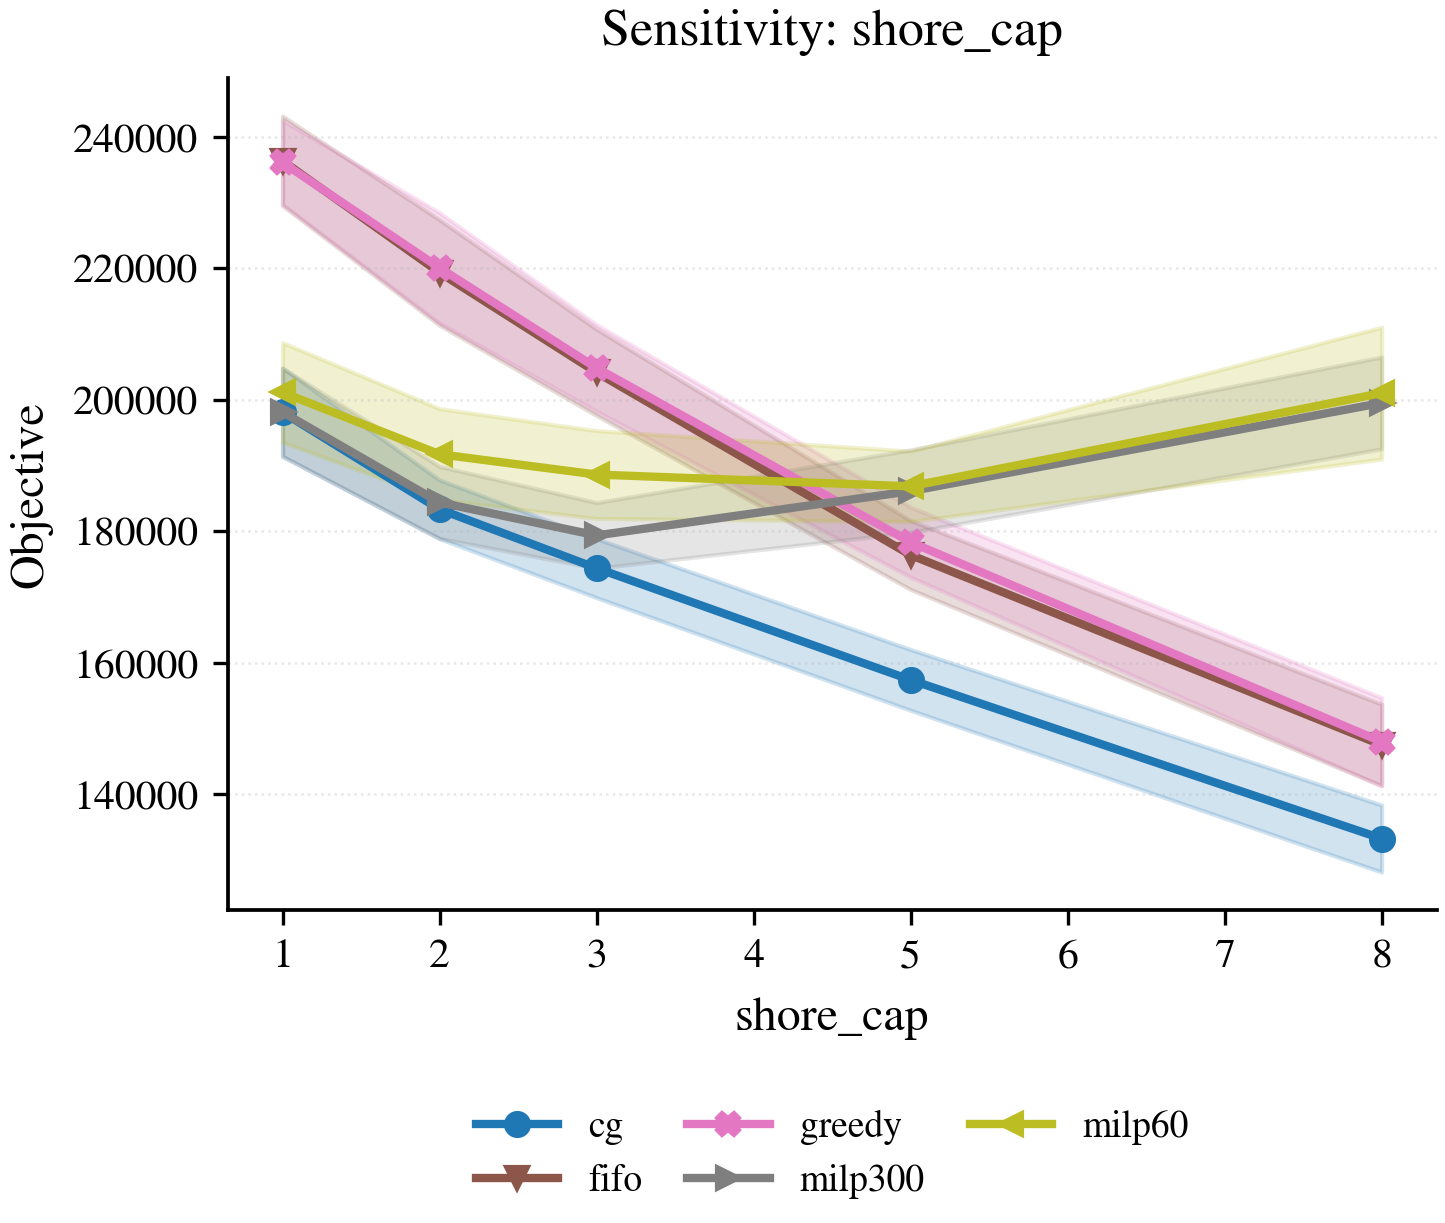
\includegraphics[width=0.85\textwidth]{figs/sensitivity/Fig_Sens_ShoreCap.png}
    \caption{岸电桩容量敏感性分析（CG）。}
    \label{fig:sens_shore}
\end{figure}

\begin{figure}[htbp]
    \centering
    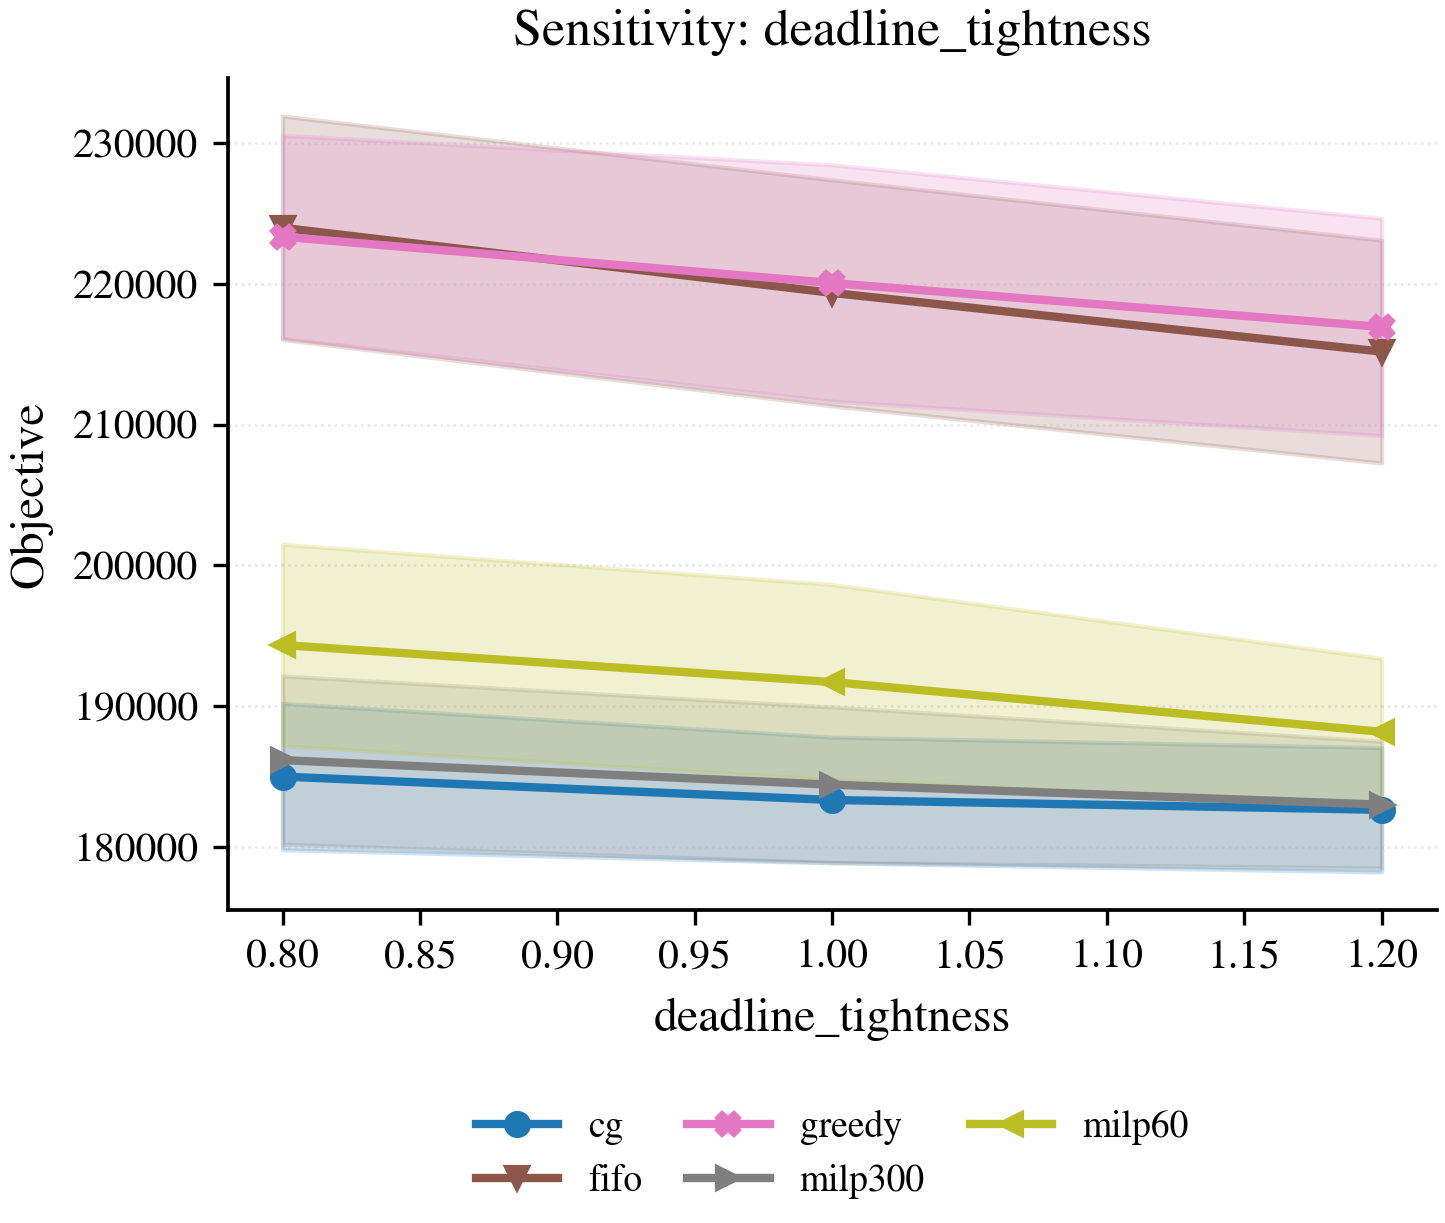
\includegraphics[width=0.85\textwidth]{figs/sensitivity/Fig_Sens_Deadline.png}
    \caption{延误紧迫度敏感性分析（CG）。}
    \label{fig:sens_deadline}
\end{figure}

\subsection{可扩展性与消融实验（可选）}
\label{sec:ablation}
为检验 CG 关键策略的作用，对 warm-start、稳定化与多列定价等变体进行消融。图 \ref{fig:ablation} 显示不同 CG 变体在目标值上完全一致，说明解质量不受策略变化影响；运行时间差异较小，表明当前定价剪枝已能提供稳定的计算效率。在本文实验规模下，基础版 CG 已足以兼顾解质量与计算成本。

\begin{figure}[htbp]
    \centering
    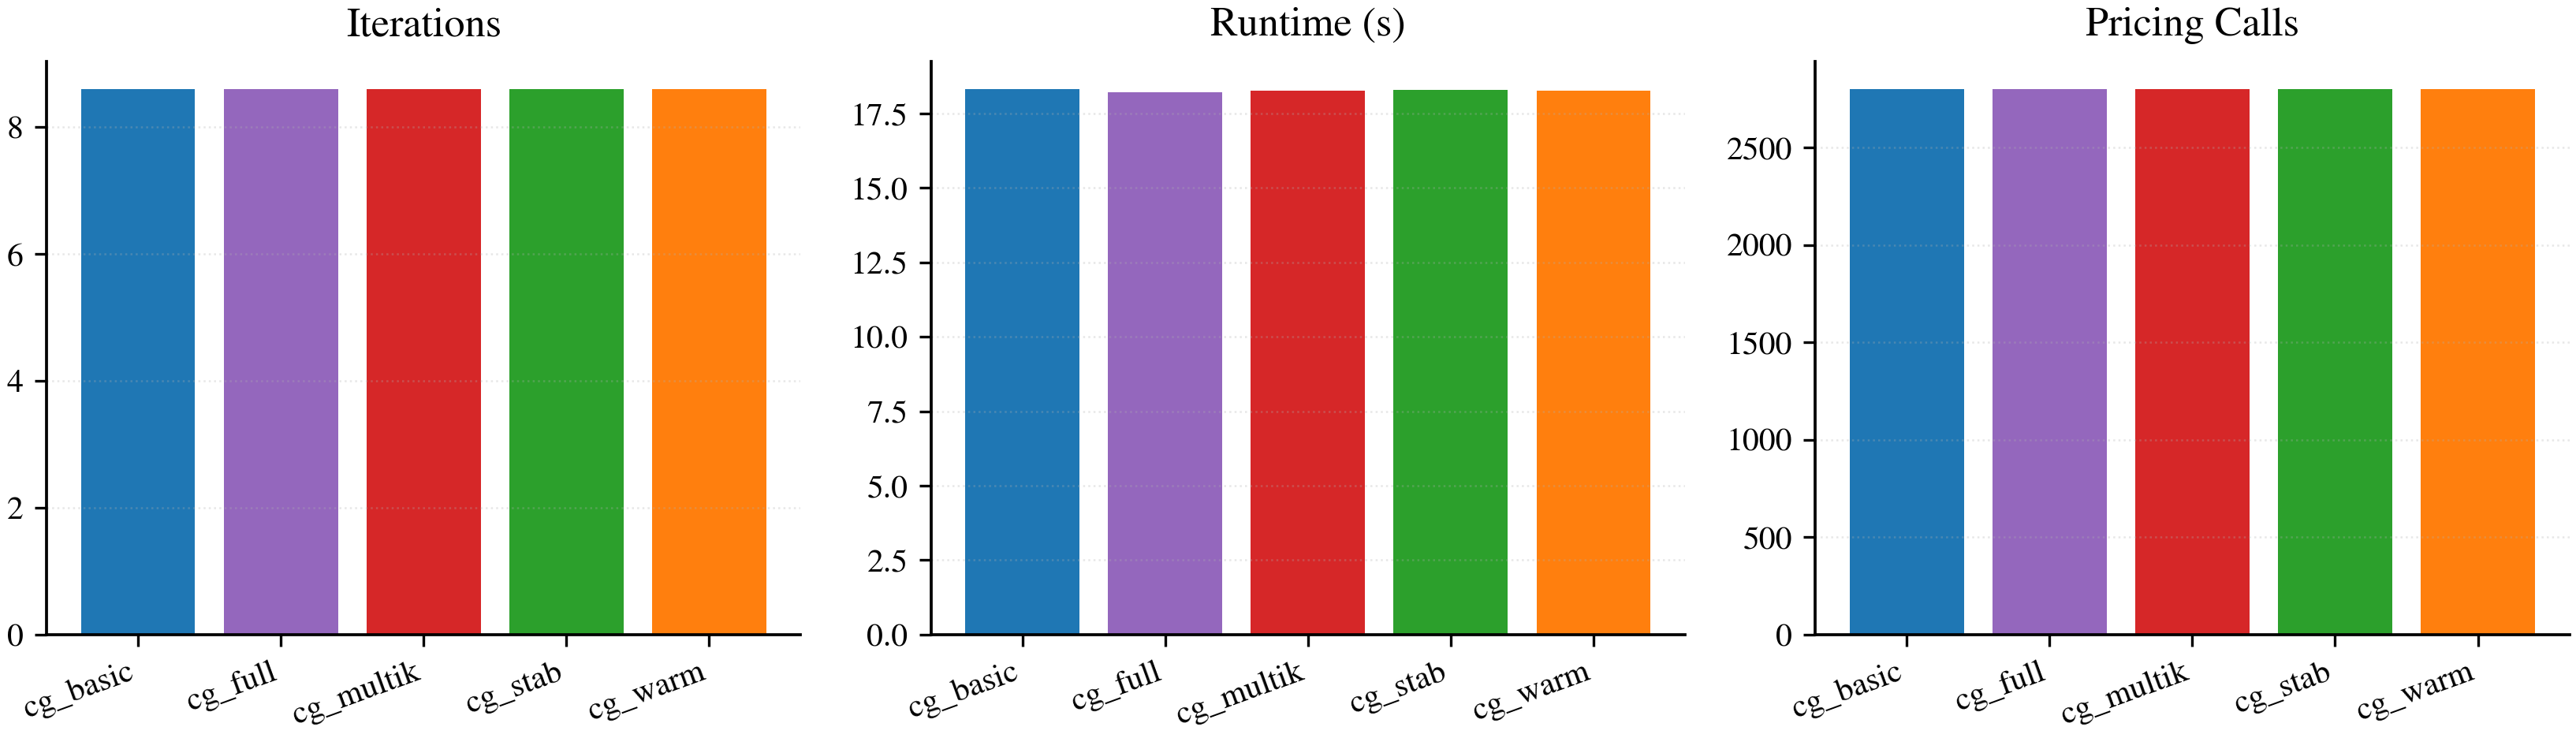
\includegraphics[width=0.8\textwidth]{figs/paper/Fig_Ablation_Bars.png}
    \caption{CG 消融结果对比。}
    \label{fig:ablation}
\end{figure}


%% --- 参考文献区 ---
\bibliographystyle{plain} % 或者使用 gbt7714-numerical
\bibliography{ref}

\end{document}
